\graphicspath{{figures/chapter3/}}
\onehalfspacing

\chapter{UAV photogrammetry for annual glacier reconstruction (2015-2023)}\label{ch:3}

\vfill

\newthought{This chapter is based on:}

\noindent Ioli, F., Bianchi, A., Cina, A., De Michele, C., Maschio, P., Passoni, D., \&
Pinto, L. (2021). Mid-Term Monitoring of Glacier’s Variations with UAVs: The Example of
the Belvedere Glacier. Remote Sensing, 14(1), 28.
\url{https://doi.org/10.3390/rs14010028}

\newpage

{\color{red} TODO: move the definition of the three sectors in discussion (experimentally bases!). Remove all references to sectors before that.}


\section{Introduction\textcolor{red}{TODO}}\label{sec:3:intro}

\textcolor{red}{TODO}


\section{Instruments and datasets\textcolor{red}{TODO}}\label{sec:3:instrument}

\textcolor{red}{Short intro to section...}

 
\subsection{GNSS measurements}\label{sec:3:gnss}

A set of GCPs was materialized with square cross targets, printed on polypropylene sheets
and anchored on big rocks (\figref{fig:3:belvedereGCP}b).
About 25 targets were deployed over the glacier (named hereafter as \textit{moving targets} or \textit{M\#} in \figref{fig:3:belvedereGCP}a) and 24 targets (labelled as 
\textit{stable targets} or \textit{S\#} in \figref{fig:3:belvedereGCP}a) were placed on
stable areas along the moraines so that they were not subjected neither to the ice flow
nor to rock falls.
Every year, the condition of each target was checked and, if one was damaged or
destroyed, the polypropylene sheet was replaced by keeping the same location of the
center (i.e., by using the same fisher plugs).
During the years, some targets were lost, and therefore new ones were materialized (e.g.,
M29bis).
Targets were yearly surveyed with dual frequency (L1/L2) geodetic quality GNSS receivers
and their coordinates were framed within the official Italian reference system ETRF2000
at the epoch 2008.0, projected in UTM 32N.
For the lower part of the glacier, where the GSM network connection was available, target
position was obtained in nRTK with respect to a network of CORS permanent stations
(either HxGN SmartNet or SPIN GNSS).
The points were occupied at least twice, each time for a duration of \qty{5}{\second}.
By contrast, in the upper part of the glacier, targets were surveyed with static sessions
of \qty{\sim 10}{\minute}, and raw observation data was post-processed with respect to
local master stations, located on stable and well known points.
To this end, either the point \textit{S12}, placed on a big rock next to the
Zamboni-Zappa hut, or the point \textit{S20}, located near the Rifugio Ghiacciai del Rosa
on the Belvedere hill,	were used (see \figref{fig:3:belvedereGCP}a).
Accuracy of GNSS measurements was evaluated empirically by comparing repeated
measurements over stable targets carried out in different years.
RMSE of \qty{1.5}{\centi\meter} in planimetry and \qty{3}{\centi\meter} in elevation were
obtained.

\begin{figure}
    \centering
    \subcaptionbox{\label{fig:3:3:studyarea:map}}{
        \includegraphics[width=.6\textwidth]{belvedereGCP.png}
    }
    \subcaptionbox{\label{fig:3:3:studyarea:pic}}{
        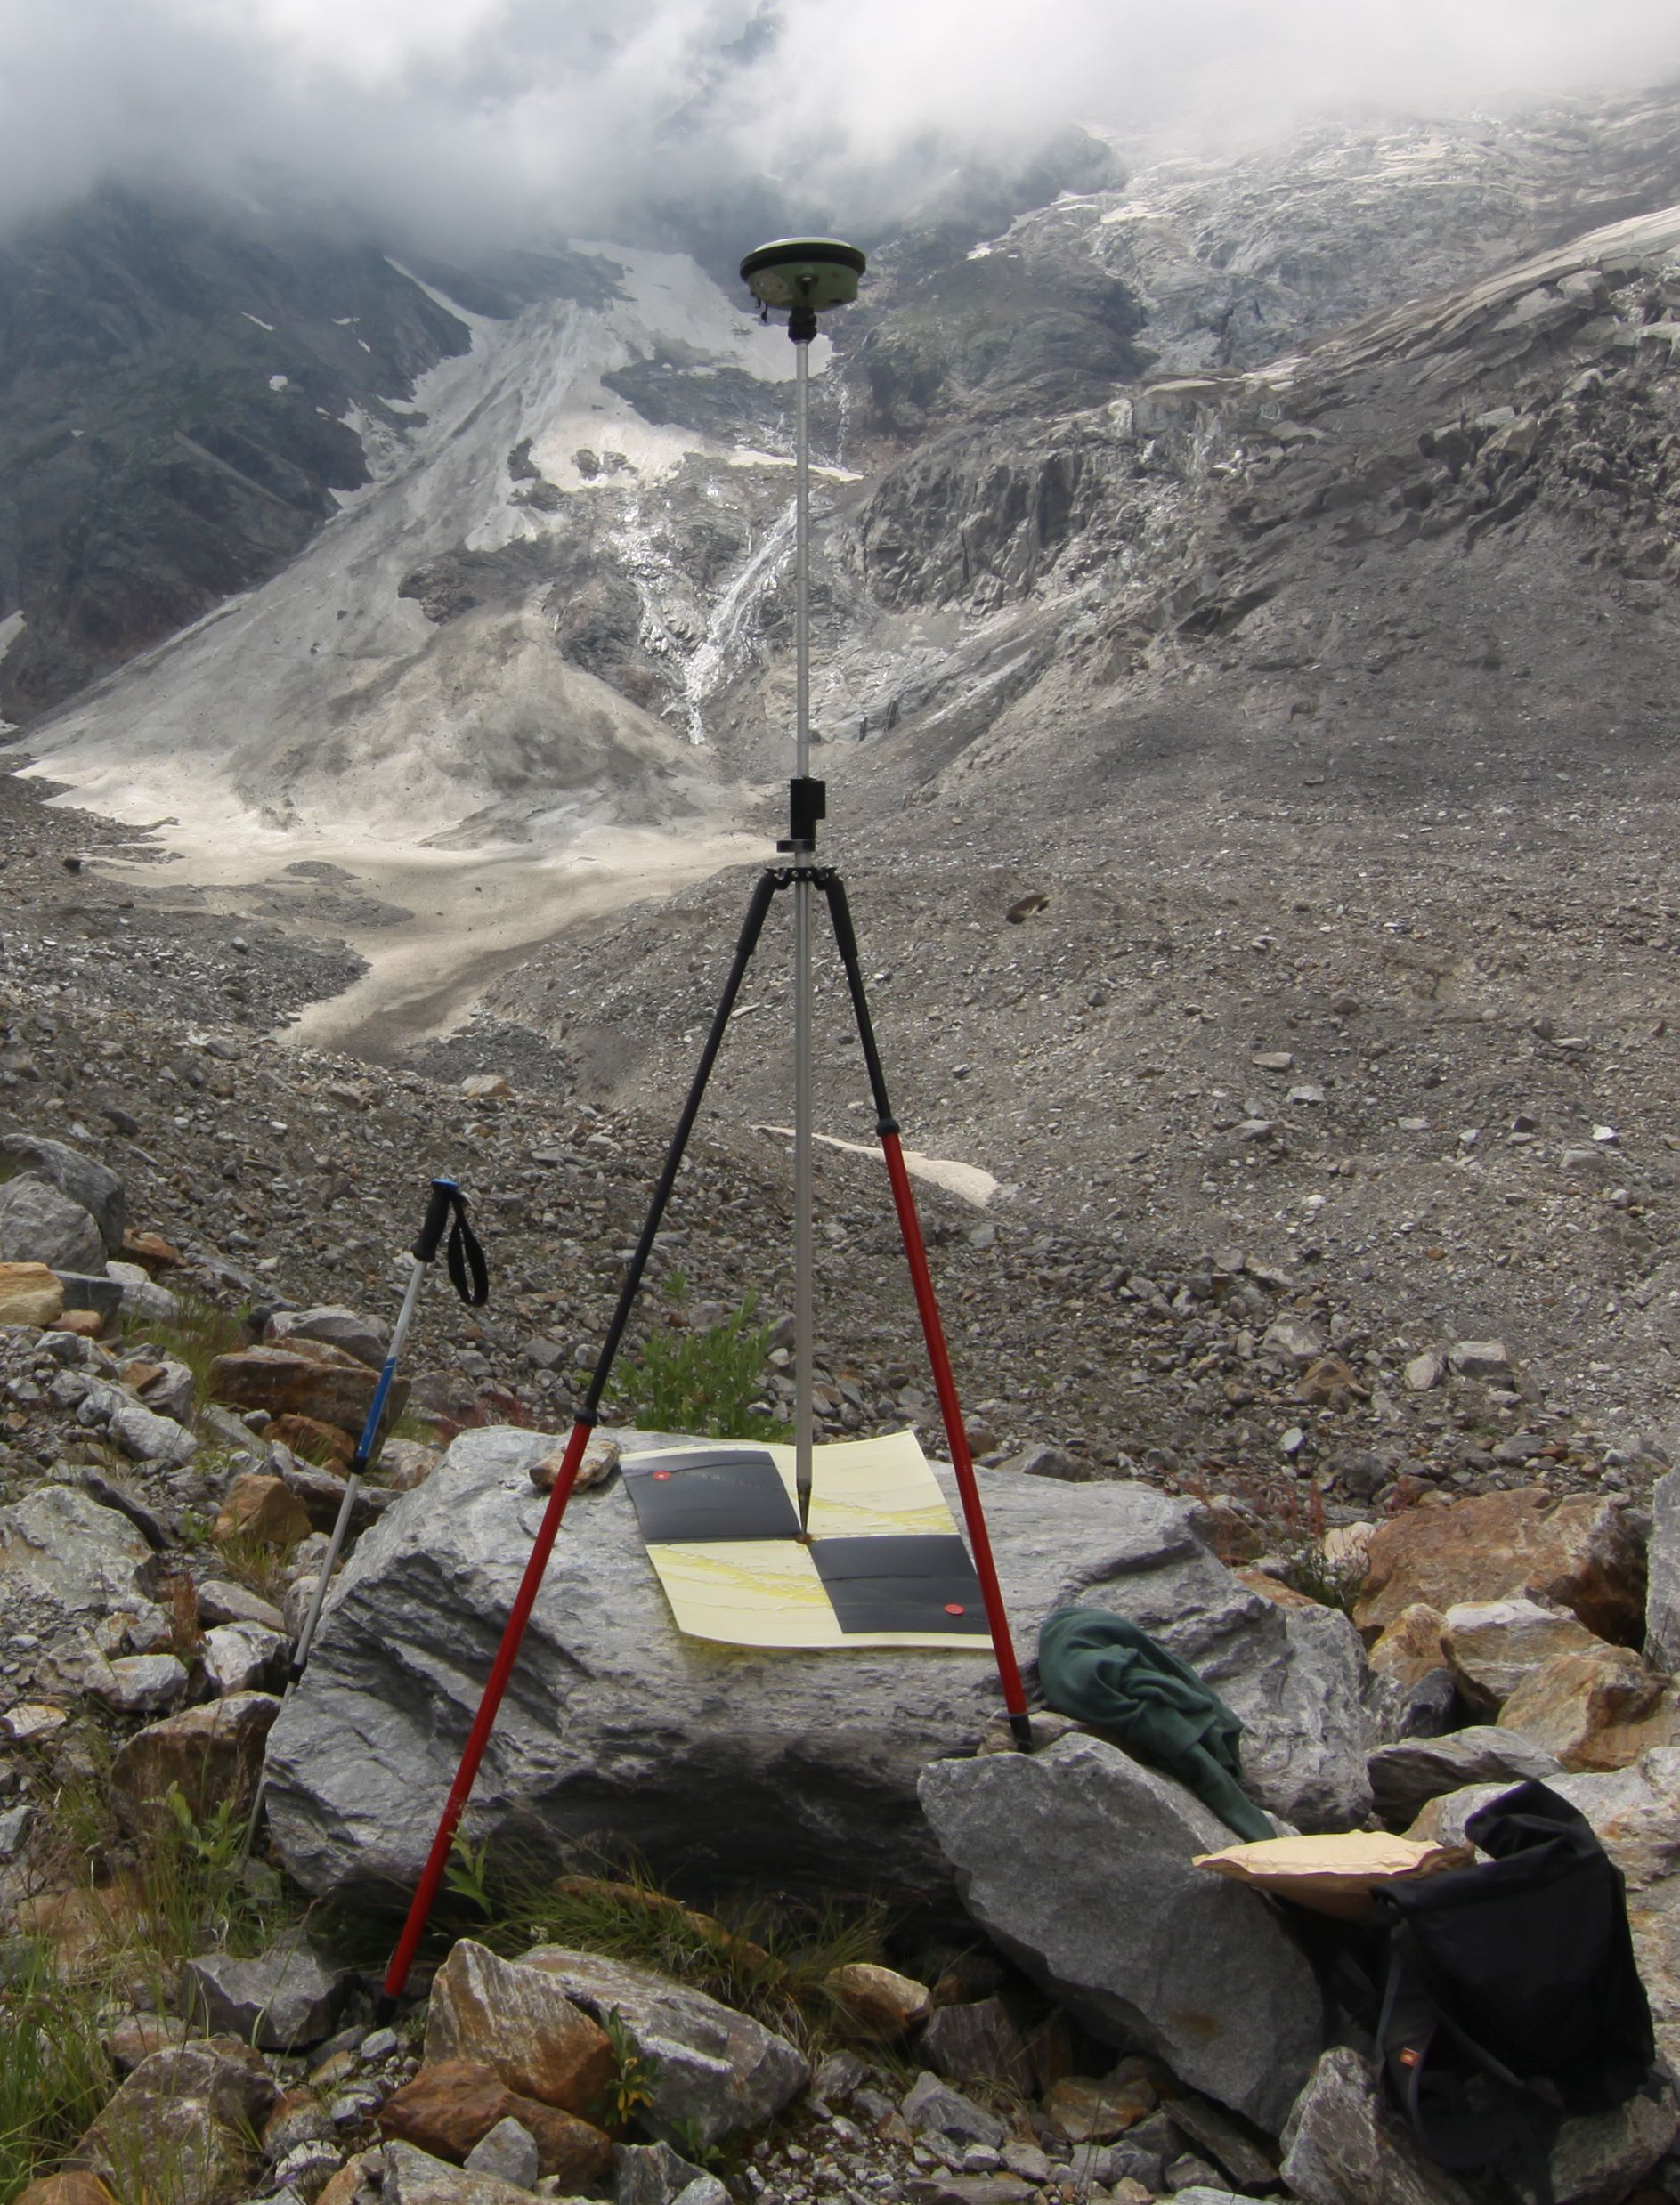
\includegraphics[width=.35\textwidth]{target.jpg}
    }
    \caption{(\textbf{a}) An example of a photogrammetric target deployed over the
        glacier moraine; (\textbf{b}) location of the targets used for the
        photogrammetric
        surveys. For~each year, a~subset of the targets were used as GCPs, while the
        remaining
        as~CPs.}
    \label{fig:3:belvedereGCP}
\end{figure}


\subsection{UAV flights\textcolor{red}{UPDATE}}\label{sec:3:uav-flights}

Because of the long duration of the monitoring campaign, the challenging environment and
the fact that more than one research group was involved in the project, different UAV
platforms and cameras were used.
As reported in \tabref{tab:3:datasets}, in~2015 and 2016, a~ready-to-fly fixed-wing UAV
SenseFly eBee, equipped with a compact camera Canon PowerShot S110, was employed to
survey the whole glacier.
During 2017, different combinations of UAVs (fixed-wing and quadcopters) and cameras were
employed (\tabref{tab:3:datasets}).
From 2018 to 2020, a~low-cost recreational fixed-wing UAV Parrot Disco FPV, with~a
wingspan of \SI{1.15}{\meter} and a weight of \SI{750}{\gram}, was adapted to carry a
small and lightweight action cam Hawkeye Firefly~8S.
For each camera, the main sensor and objective characteristics are listed
\tabref{tab:3:camere}.

UAVs flights were conducted automatically by using ground station software packages
developed by UAV manufacturers.
    {\color{red} Add UGCS...}

The flights were designed to have GSD ranging between \qtylist{5;10}{\centi\meter}, and
to guarantee \qty{\sim 80}{\percent} of longitudinal and \qty{\sim 60}{\percent} of
transversal overlap.
Average image GSD values and number of GCPs and CPs, used respectively to orient the
images and to assess the quality of the photogrammetric blocks, are summarized in
\tabref{tab:3:datasets}.

{\color{red} Add instruments for 2021-2023...}

\begin{table}[p]
    \small
    \centering
    \caption{Summary of the characteristics of the surveys.}
    \begin{tabular}{c  m{1.8cm} m{3.5cm} m{4.2cm} c c c }
        \toprule
        Year                                                              & Date
                                                                          & UAV
                                                                          & Camera
                                                                          & GSD
                                                                          & GCP
                                                                          & CP
        \\
                                                                          &
                                                                          &
                                                                          &
                                                                          & [m/px]
                                                                          & [\#]
                                                                          & [\#]
        \\
        \midrule
        2015                                                              & A.
        8.10\newline B. 23.10                                             &
        SenseFly eBee                                                     & Canon
        PowerShot S110                                                    & 0.07
                                                                          & 24
                                                                          & 11
        \\[4mm]
        2016                                                              & 20.10
                                                                          & SenseFly eBee
                                                                          & Canon
        PowerShot S110                                                    & 0.09
                                                                          & 31
                                                                          &
        15
        \\[4mm]
        2017                                                              & A.
        5.10\newline B. 15.11\newline C. 16.11                            & A. SenseFly
        eBee \newline B. SenseFly eBee Plus\newline  C. DJI Phantom 4 Pro & A. Canon
        PowerShot
        S110  \newline B. SenseFly S.O.D.A \newline C. DJI FC6310         & 0.06
                                                                          & 27
                                                                          & 8
        \\[4mm]
        2018                                                              & 23-25.07
                                                                          & Parrot Disco
                                                                          & Hawkeye
        Firefly 8S                                                        & 0.05
                                                                          & 27
                                                                          &
        13
        \\[4mm]
        2019                                                              & 29.07-2.08
                                                                          & Parrot Disco
                                                                          & Hawkeye
        Firefly 8S                                                        & 0.06
                                                                          & 26
                                                                          &
        10
        \\[4mm]
        2020                                                              & A. 26-27.07
        \newline B. 9.08                                                  & A.
        Parrot Disco\newline B. DJI Phantom 4 Pro                         & A. Hawkeye
        Firefly 8S\newline B. DJI FC6310                                  &
        0.05                                                              & 29
                                                                          & 12
        \\[4mm]
        2021                                                              & 29.07-2.08
                                                                          & DJI Matrice 210 V2
                                                                          & DJI ZenMuse x5s
                                                                          & 0.04
                                                                          & 23
                                                                          &
        9
        \\[4mm]        
        2022                                                              & 28.07-29.07
                                                                          & DJI Matrice 300 RTK
                                                                          & DJI Zenmuse P1 - 35 mm
                                                                          & 0.03
                                                                          & 22
                                                                          &
        19
        \\[4mm]
        2023                                                              & 25.07-27.07
                                                                          & DJI Matrice 300 RTK
                                                                          & DJI Zenmuse P1 - 35 mm
                                                                          & 0.03
                                                                          & XX
                                                                          &
        XX
        \\[4mm]        
        \bottomrule

    \end{tabular}
    \label{tab:3:datasets}
\end{table}

\begin{table}[p]
    \centering
    \small
    \caption{Summary of the characteristics of the cameras employed.}
    \begin{tabular}{c c c c c c}
        \toprule
        Camera                        & Sensor                        & Sensor Size
                                      & Focal length                  & Image size
                                      & Pixel size
        \\
                                      &                               &
        [\SI{}{\milli\meter\squared}] & \newline[\SI{}{\milli\meter}] & [\SI{}{\pixel}]
                                      & \newline[\SI{}{\micro\meter}]
        \\

        \midrule
        Canon PowerShot S110          & 1/1.7" CMOS                   & $7.44\times5.58$
                                      & 5.2                           & $ 4000 \times
            3000
        $                             & 1.9
        \\
        SenseFly S.O.D.A              & 1" CCD                        & $13.2\times8.8$
                                      & 10.6                          & $5472 \times
        3648$                         & 2.4
        \\
        DJI FC6310                    & 1" CMOS                       & $13.2\times8.8$
                                      & 8.8                           & $5472 \times3648$
                                      & 2.4
        \\
        Hawkeye Firefly 8S            & 1/2.3" CMOS                   & $6.17\times4.56$
                                      & 3.8                           & $5472 \times3648$
                                      &
        1.34
        \\
        DJI ZenMuse x5s               & 4/3" CMOS                     & $17.3\times13$
                                      & 15                            & $5280 \times
        3956$                         & 3.3 
        \\
        DJI Zenmuse P1 - 35 mm        & FullFrame CMOS                & $35.9\times24$
                                      & 35                            & $8192 \times
        5460$                         & 4.4
        \\
        \bottomrule
    \end{tabular}
    \label{tab:3:camere}
\end{table}

\subsection{Problems Arisen during the surveys of 2017 and~2020 {\color{red} REVISE}} \label{sec:3:problems} 
% Compared to traditional glaciological techniques, UAVs allow for a significant reduction of in-situ operations (limited to surveying few GCPs spread along the glacier and performing UAV flights).
Conducting a yearly monitoring campaign in an alpine environment for~six consecutive
years is challenging because of, for example,~the hard accessibility of some areas of the
glacier (also for fixed-wing UAVs take-off and landing) and the variability of the
meteorological~conditions.

Adverse meteorological conditions and practical issues made it necessary to split the
2017 survey in different dates, and~various UAVs and cameras were employed (see
\tabref{tab:3:datasets}).
The 2017 photogrammetric model was therefore divided into three parts: the central part
refers to the October survey while the lower and the upper parts refer to the November
survey and at that time the glacier was covered by snow (\figref{fig:3:ortophoto}c).
Technical problems arose also during the 2020 survey: a breakage of one elevon servo
during a landing phase caused the fixed-wing UAV to crash.
Therefore, a~quadcopter DJI Phantom 4 Pro was employed to survey the upper part of the
glacier (approximately the S1 sector, see the different colors in the orthophoto of
\figref{fig:3:ortophoto}f) 14 days after the former.
However, during~the August 2020 fieldwork, it was not possible to measure any additional
GCPs because the south-west part of the Belvedere Glacier, close to the Monte-Rosa
Glacier is hardly accessible and dangerous due to the presence of crevasses and steep
rocks.
The few GCPs available in the upper part of the glacier made necessary to co-register the
Phantom 4 Pro model on the 2019 model, by~searching for sharp edges of rocks along the
moraines, remained fixed along the year, on~ 2019 images.
This approach is less accurate than measuring targets directly on the field.
The RMSE on CPs was therefore equal to \SI{0.36}{\meter} (see
\figref{fig:3:CP_errors}), \SI{\sim 7}{}~times the GSD.
Nevertheless, the~area affected by this issue was rather limited, compared to the whole
Belvedere~Glacier.

Moreover, between~2017 and 2018, the~survey period was moved from Autumn to Summer.
From 2015 to 2017, in~fact, field works were included within the DREAM project (see
\secref{sec:3:intro}) and they took place in Autumn, at~the beginning of the academic
year.
By contrast, from~2018 to 2020, surveys were carried out at the end of July because they
were encompassed within a Summer School organized by DICA (Politecnico di Milano).
The change in the survey dates was critical because the timespan occurred between the
survey of October/November 2017 and that of July 2018 did not include the period of
maximum ablation and velocity of the glacier (neither August 2017 nor August 2018).
Therefore, volume variation and ice flow velocity refer mostly the wintertime and the
results obtained are not directly comparable with those of the other~years.


\section{Metodology}\label{sec:3:methodology}

\subsection{SfM workflow}\label{sec:3:sfm}

In order to build photogrammetric models of the glacier, images acquired during UAV
surveys were processed with the SfM software Agisoft Metashape 1.7.2 \citep{agisoft}.
For each year, at least 24 GCPs spread over the glacier were employed to orient the
images, whereas at least 10 Check Points (CPs) were used to assess models quality.
Both GCPs and CPs were manually collimated on the images.
Tie Points (TPs) were detected and matched by Metashape on full resolution images (which
corresponds to \textit{high accuracy} parameter in Metashape).
Image External Orientation (EO) and TPs world coordinates were estimated by solving the
Bundle Block Adjustment (BBA).
TPs with the worst reprojection error on images, which are likely originated from false
matches, were removed and the BBA was solved again to improve quality of BBA solution.
This process was iterated more times until TPs mean reprojection error had dropped below
\SI{\sim 0.8}{\pixel}.
Camera internal orientation was estimated by self-calibration
\citep{Fraser2013,Cramer2017}, because of its instability in the cameras employed.

Dense 3D reconstruction was computed by Agisoft Metashape with proprietary MVS
algorithms~\citep{Dallasta}.
Depth maps and dense point clouds were obtained from images downsampled by a factor 4,
in~order to reduce the computational time (\textit{medium quality} parameter of the dense
cloud generation in Metashape).
Triangulated mesh surfaces and photorealistic textures were~computed.

DSMs with a resolution of \SI{0.5}{\meter\per\pixel} were derived from the mesh model.
Finally, orthophotos with a GSD of \SI{0.10}{\meter\per\pixel} were obtained by
projecting the most nadiral images over the mesh model (\figref{fig:3:ortophoto}).

\subsection{Glacier flow velocity\textcolor{red}{TODO}}\label{sec:3:method_velocity}

In case of debris-covered glacier, big rocks and boulders usually move jointly with the ice flow \textcolor{red}{REF}, 
Therefore, it was possible to investigate ice flow dynamics and to estimate glacier surface velocity by evaluating debris pattern movements.
In-situ GNSS measurements of the \textit{moving targets}, deployed over big rocks (see~\secref{sec:3:gnss}),  were first employed to estimate yearly average velocities of the glacier.
Targets coordinates, measured on different years, were differentiated and the annual average velocity of each point was derived by dividing the displacement by the time lag. 
These punctual velocity measurements are hereafter labelled as \textit{GNSS} and they can be considered as high accurate (i.e., centimetric) measurements of glacier displacements and velocities.

{\color{red} ADD DIC}

The number of GNSS measurements are limited to a dozen of points spread over the glacier, consequently they are not enough to derive a complete glacier velocity field.
Hence, DIC algorithms, such as normalized cross-correlation or orientation correlation~\citep{Heid2012_evaluation_xcorr} are widely applied to automatically compute displacement on orthophotos and might allow for sub-pixel accuracy \citep{Debella_Gilo2011}.	

{\color{red} motivate MAN because of snow and validation of DIC}

Additionally, a set of features were manually collimated on orthophotos and tracked over the years to obtain complete surface velocity fields.
These points are named as \textit{MAN}.

However, because of the presence of snow and due to significantly different environmental conditions between years (\figref{fig:3:ortophoto}), it was not feasible to apply automatic image matching algorithms on all the orthophotos to obtain displacements between corresponding pattern of pixels. 
Therefore, the visual collimation of characteristic features (e.g., sharp edges of big rocks emerging from the snow) on different orthophotos was the only possibility to track elements on the glacier surface. 
Even though manual collimation precision of natural elements, such as rocks, on orthophotos was likely worse compared to computer vision algorithms, a human operator supervision ensured high matching reliability.
Moreover, it was possible to define a regular grid of \qtyproduct{100 x 100}{\metre} on the orthophotos in order to select homogeneously distributed features (\qty{\sim 1}{\pt} every \qty{10000}{\meter\squared}), resulting in a total of \qty{\sim 130}{points}.
Most of the points were tracked over the years; however some were lost and only \qty{115}{points} were found on the 2020 orthophoto.


\subsection{Volume variations}\label{sec:3:method_volumes}

To compute glacier volume variation $ \Delta V $, consecutive DSMs were differentiated
by~employing a DEM of Difference (DOD) approach with the tool \textit{Compute 2.5D volume} implemented in CloudCompare~\citep{cloudcompare}.
First, photogrammetric dense clouds were gridded by projecting points along the vertical
direction on a planar surface, obtaining DSMs with a cell footprint on ground of \qtyproduct{0.5x0.5}{\meter}.
The choice of the raster resolution was a compromise to achieve a robust height field
estimation by averaging a large enough number of points for each cell of the raster,
but~at the same time small enough to maintain a spatial resolution able to map small
scale glacier morphology.
A mask was manually created and applied to all the DSMs to exclude areas outside the
glacier surface.
DSMs from consecutive years were then differentiated pixel-by-pixel to obtain the height
difference at each cell of the raster.

In order to rigorously estimate volume variation variances, by~propagating the variance,
it would be  necessary to know the covariance matrix of each DSM, considered as a
multivariate random variable with dimension equal to the number of cells.
However, no information concerning cells covariances was provided by the SfM software
employed, thus it was troublesome to compute covariances between nearby cells in a DSM
(which are clearly correlated because they were generated by the same set of images in
the photogrammetric process).
As a consequence, only a rough estimation of the variance was carried out by considering
each DSM as a mono-dimensional random variable with variance equal to the squared value
of the vertical component of RMSE computed on the CPs of the relative photogrammetric
model.
Moreover, $ DSM^{(i+1)} $ and $ DSM^{(i)} $ were considered as independent because there
was no relation between the surveys.
The variance of the volume variation was therefore computed as:
\begin{equation}
    \sigma^2_{\Delta V^{(i+1,i)}}  = {(n \times A_c)}^2 \left( \sigma^2
    _{DSM^{(i+1)}} + \sigma^2_{DSM^{(i)}} \right),
    \label{eq:3:volVarProp}
\end{equation}
where $ n $ is the number of cell in the~DSMs and $ \sigma^2 _{DSM}$ is the squared
vertical error of the photogrammetric model evaluated on the GCPs.

For the years 2015--2016, 2016--2017, 2017--2018, the~glacier was partially covered by
snow (see \figref{fig:3:ortophoto}a--c), which introduced additional uncertainties in
volume estimation.
The snow height accumulated at the nivometric station located near Zamboni Zappa Hut
(\SI{2075}{\masl}, in the central sector of the glacier) on the survey dates was retrieved
from the meteorological database of ARPA Piemonte, the regional agency for the
environment~\citep{arpaPie}: \SI{22}{\centi\meter} of snow were measured on 23 October
2015, \SI{20}{\centi\meter} on 20 October 2016, \SI{40}{\centi\meter} on 15 November 2017.
The measured snow heights were considered additional components of the DSM standard
deviations.
Yet, because the glacier was only partially covered by snow, the snow-driven uncertainty
was weighted by half of the total glacier area in variance propagation.

\subsection{Glacier outline\textcolor{red}{TODO}}\label{sec:3:method_outline}

{\color{red} TODO}

\section{Results}\label{sec:3:res}

\subsection{SfM\textcolor{red}{UPDATE}}\label{sec:3:res:sfm}

\begin{figure}
    \centering
    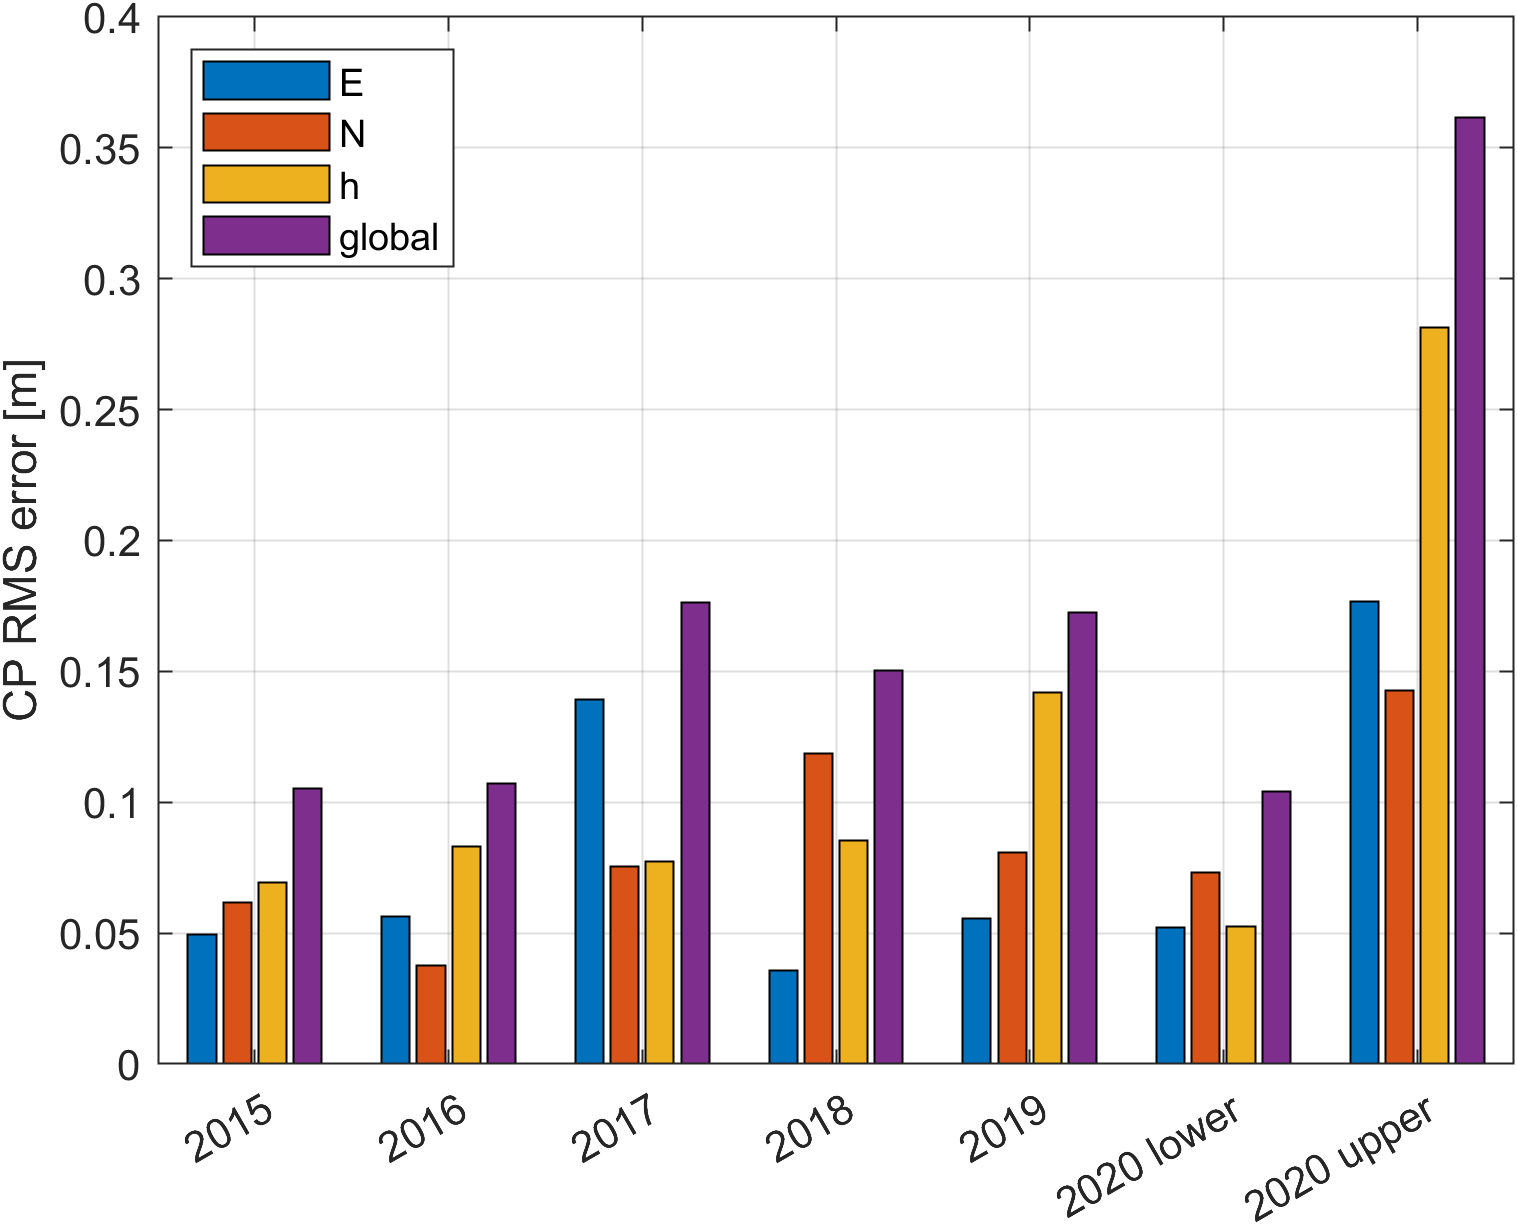
\includegraphics[width=0.7\columnwidth]{CPrmse.png}
    \caption{Barplot of reprojection RMSE computed CPs for each photogrammetric
        model. Due to practical problems occurred in 2020 and explained in
        \secref{sec:3:problems}, the~RMSE of 2020 model was split in two parts:
        \textit{2020 lower} denotes the CP RMSE over related to the central and 
        lower sectors of the glacier (S2 and S3 in \figref{fig:3:belvedere}a), 
        whereas \textit{2020 upper} refers to the upper accumulation sector 
        only (S1). {\color{red} remove 2020 upper and add recent years}}
    \label{fig:3:CP_errors}
\end{figure}

\begin{figure}
    \centering
    \subcaptionbox{\label{fig:3:ortophoto:2015}}{
        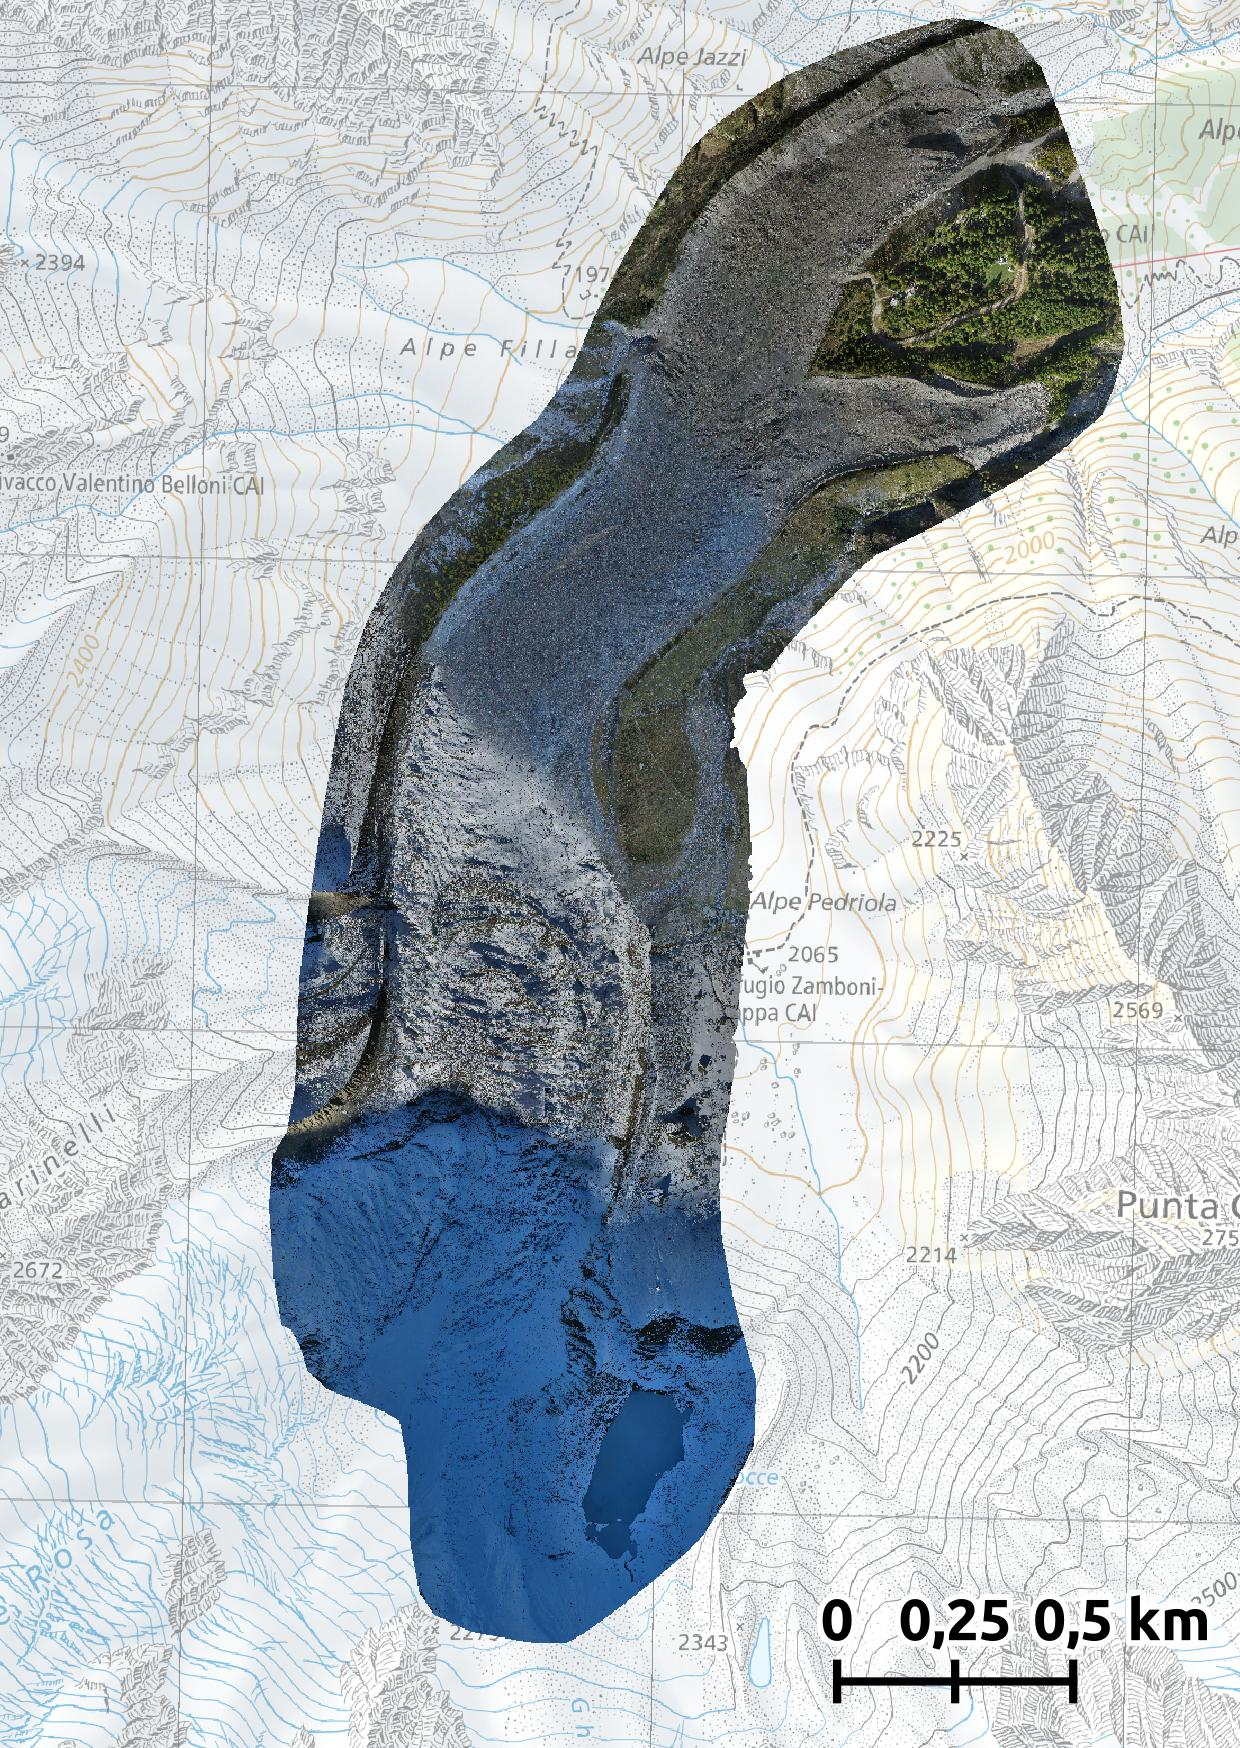
\includegraphics[width=0.30\textwidth]{orto2015.jpg}
    }
    \subcaptionbox{\label{fig:3:ortophoto:2016}}{
        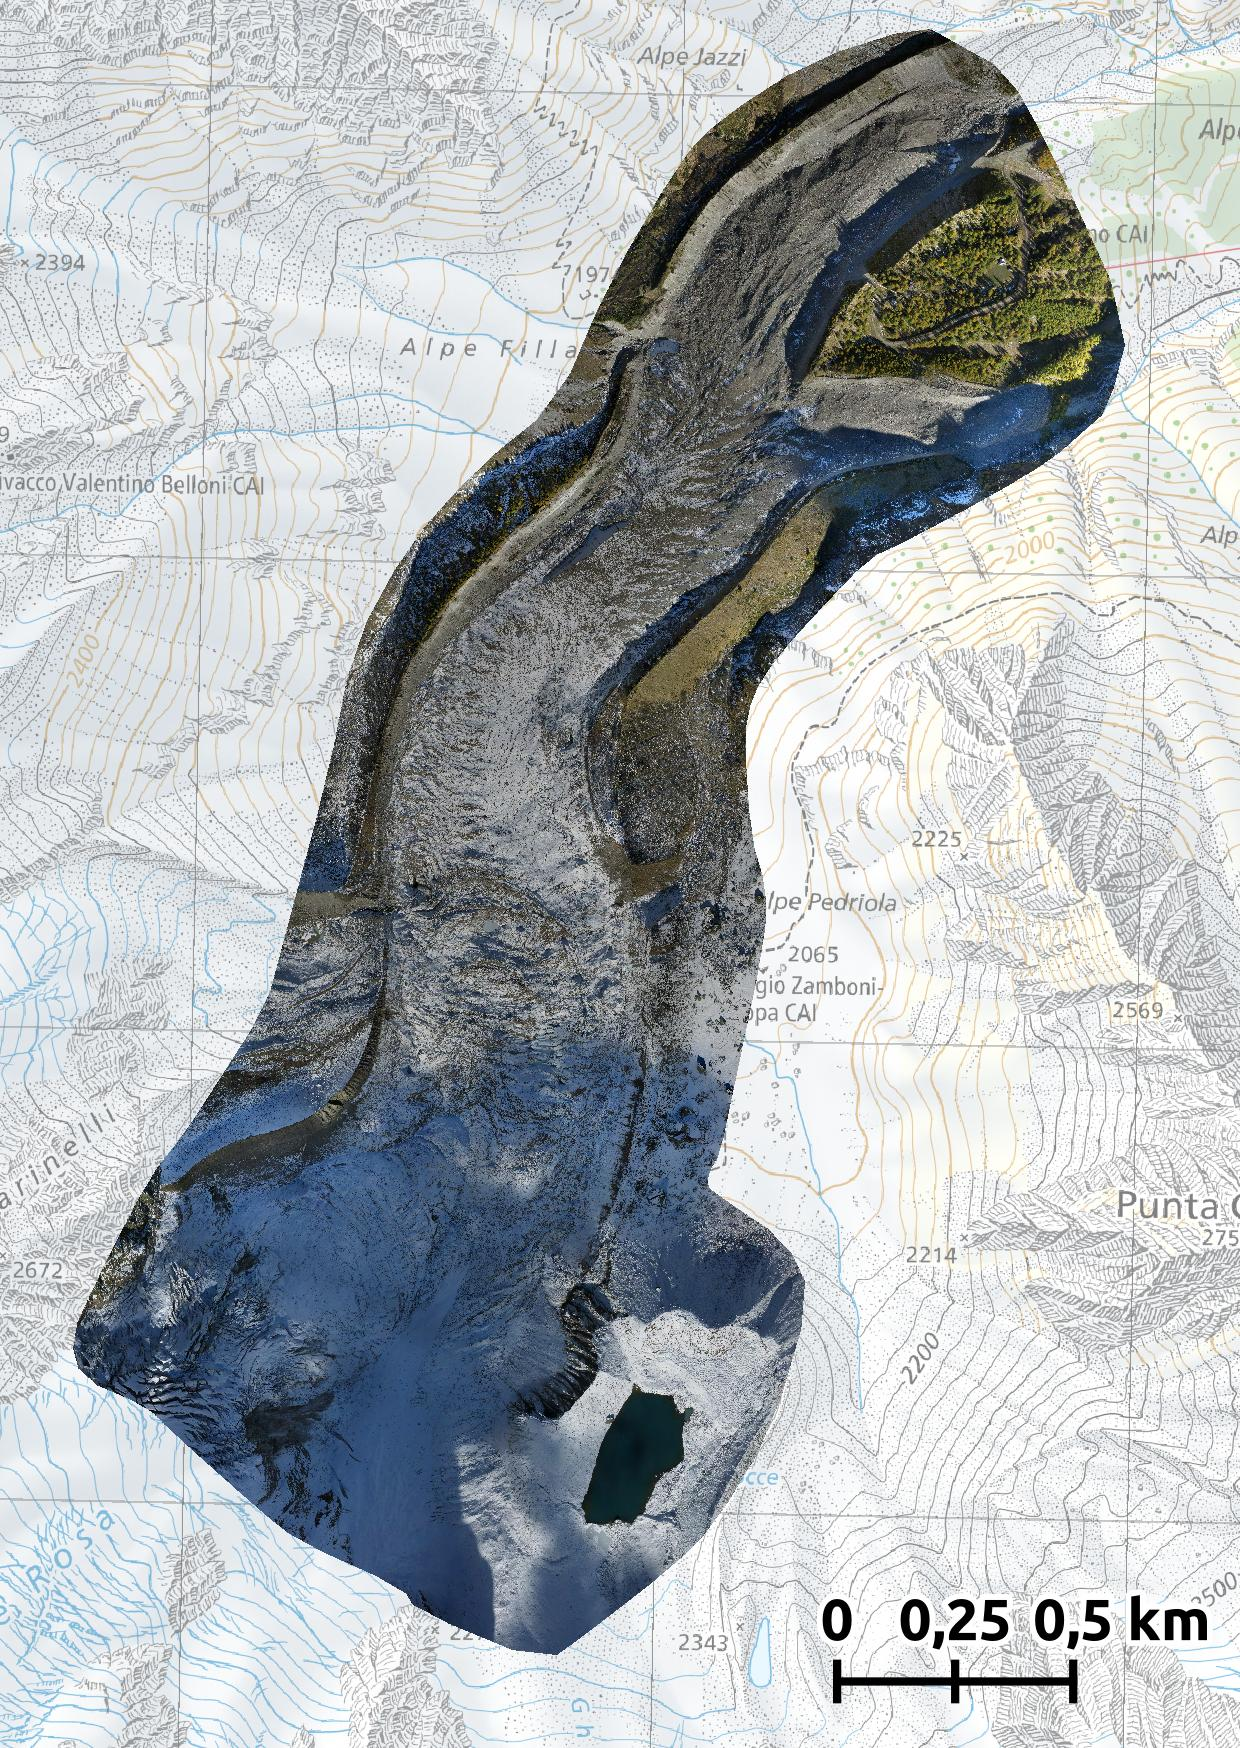
\includegraphics[width=0.30\textwidth]{orto2016.jpg}
    }
    \subcaptionbox{\label{fig:3:ortophoto:2017}}{
        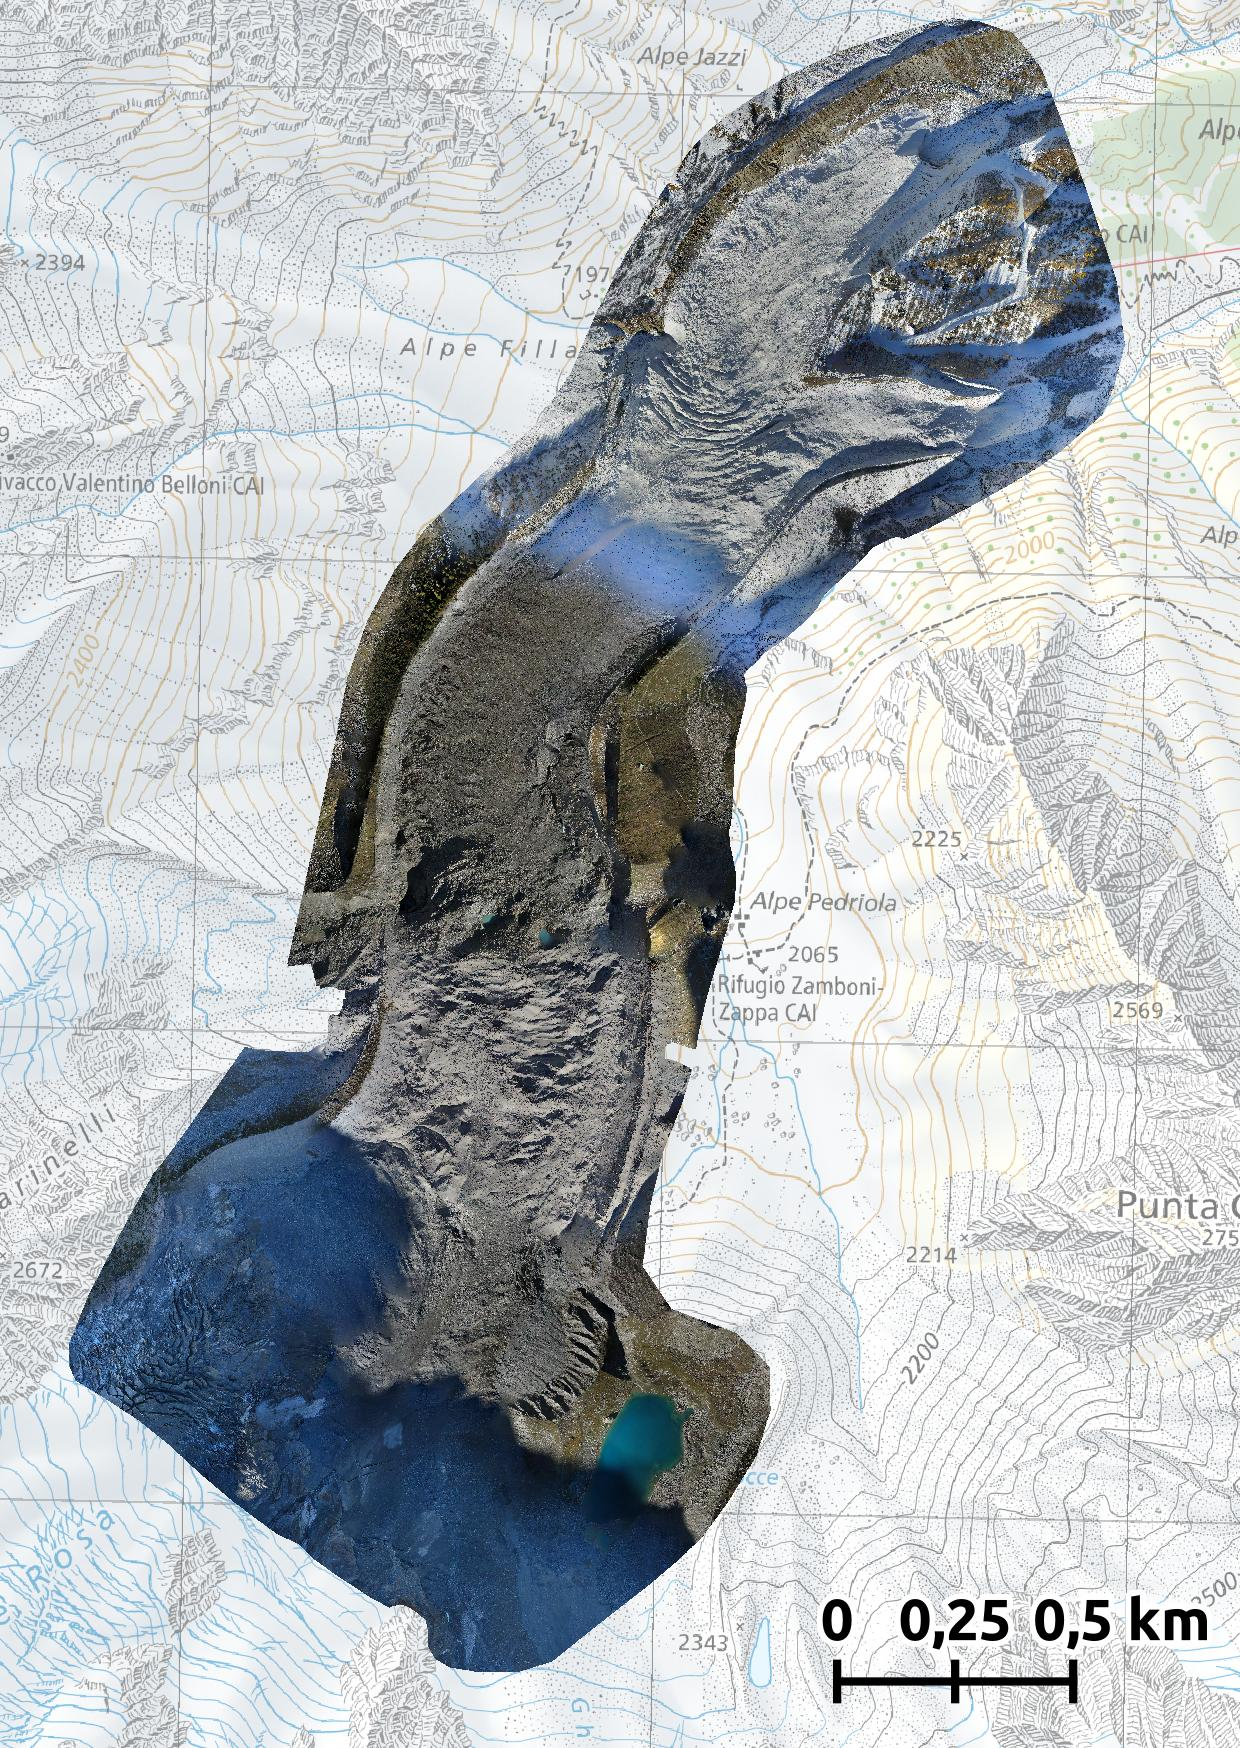
\includegraphics[width=0.30\textwidth]{orto2017.jpg}
    }
    \\
    \subcaptionbox{\label{fig:3:ortophoto:2018}}{
        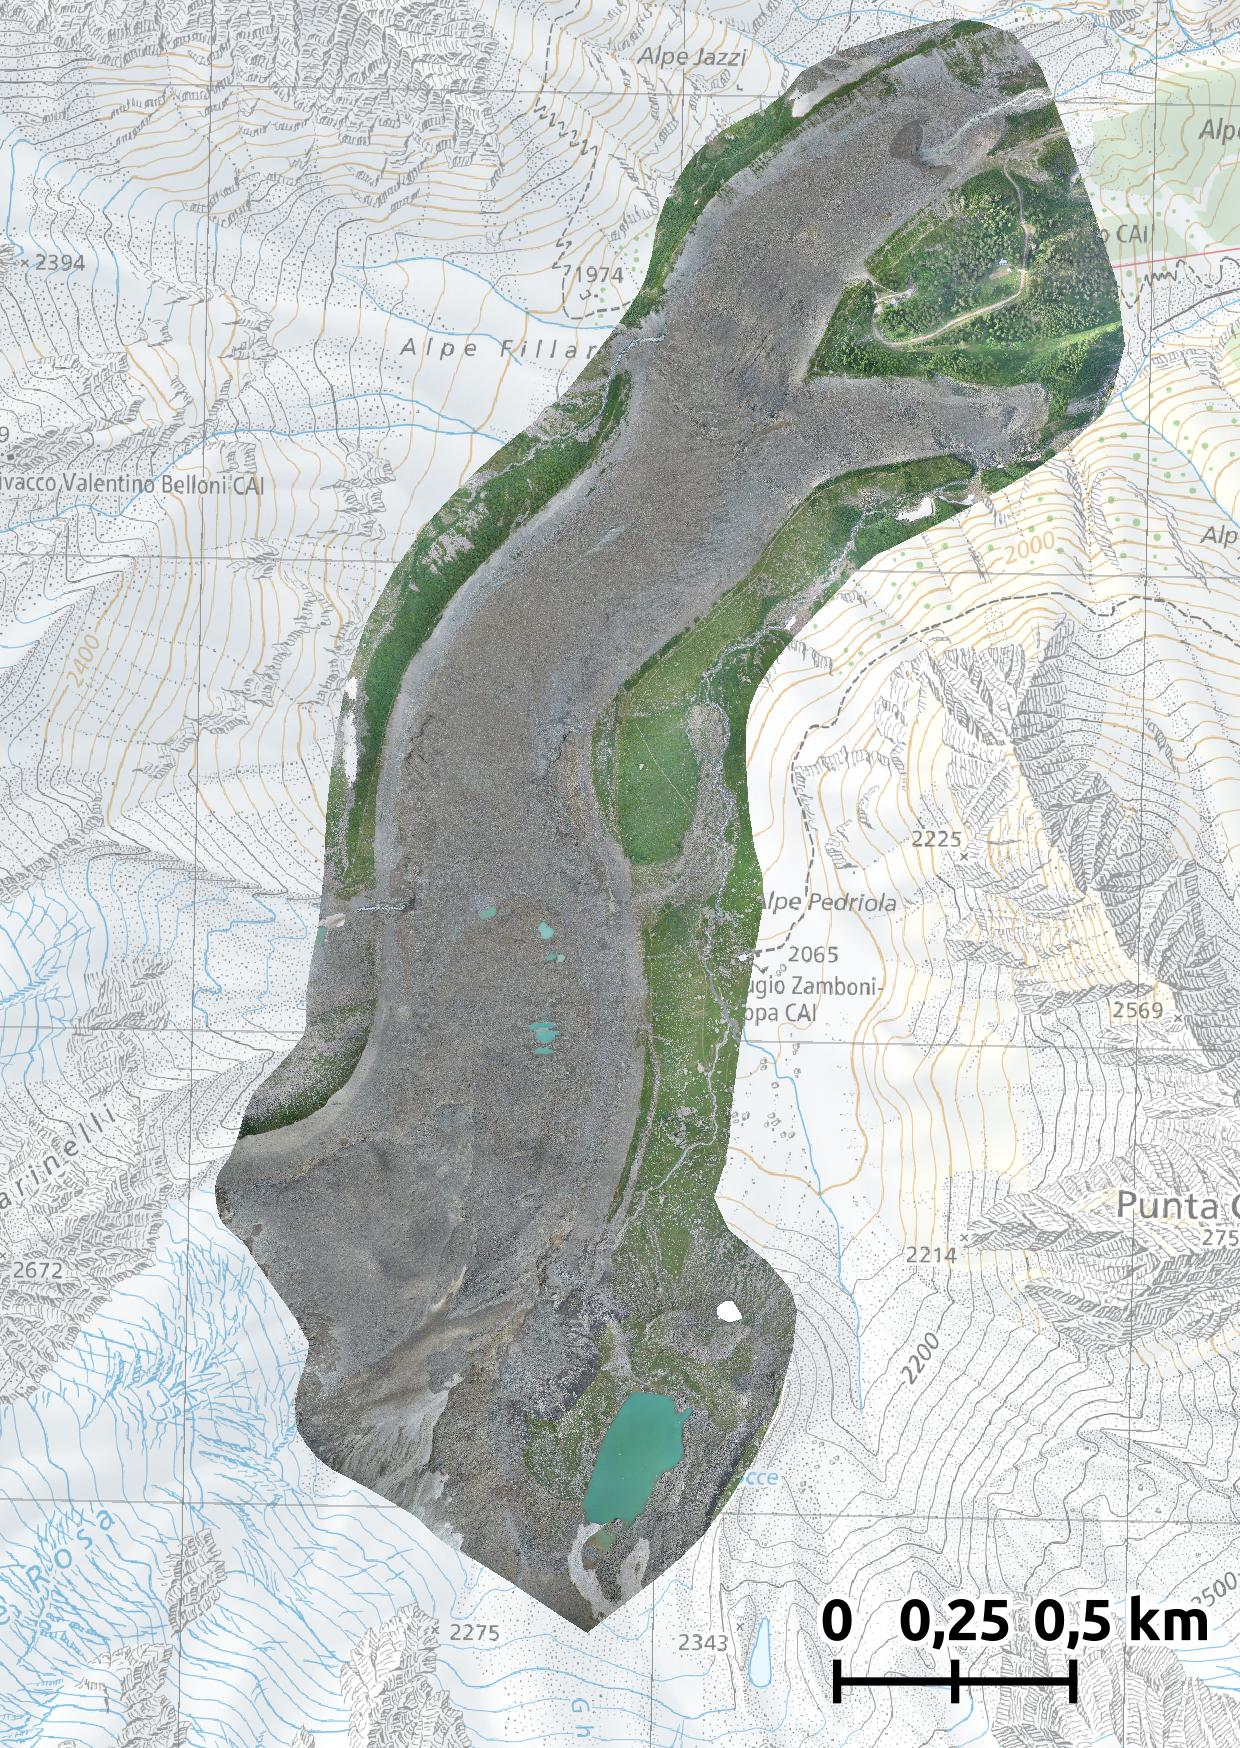
\includegraphics[width=0.30\textwidth]{orto2018.jpg}
    }
    \subcaptionbox{\label{fig:3:ortophoto:2019}}{
        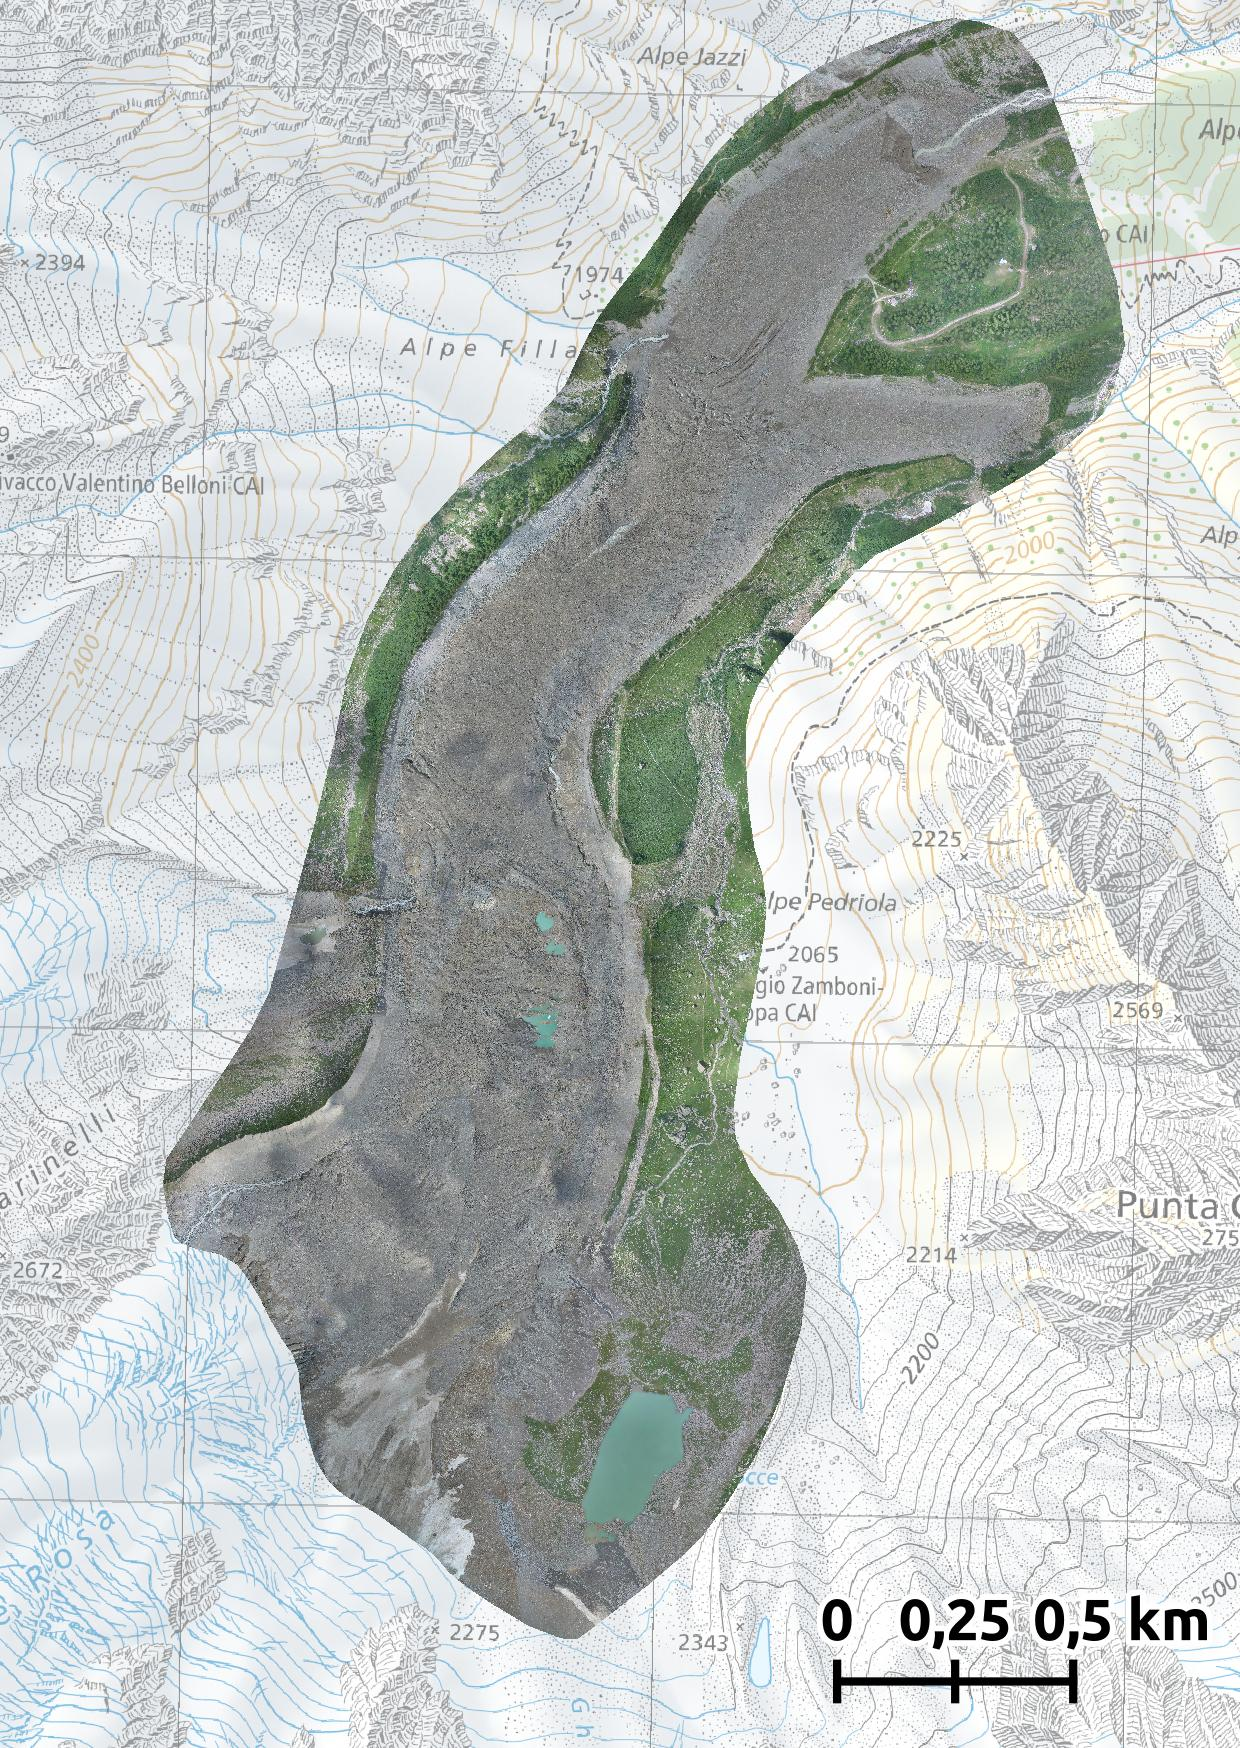
\includegraphics[width=0.30\textwidth]{orto2019.jpg}
    }
    \subcaptionbox{\label{fig:3:ortophoto:2020}}{
        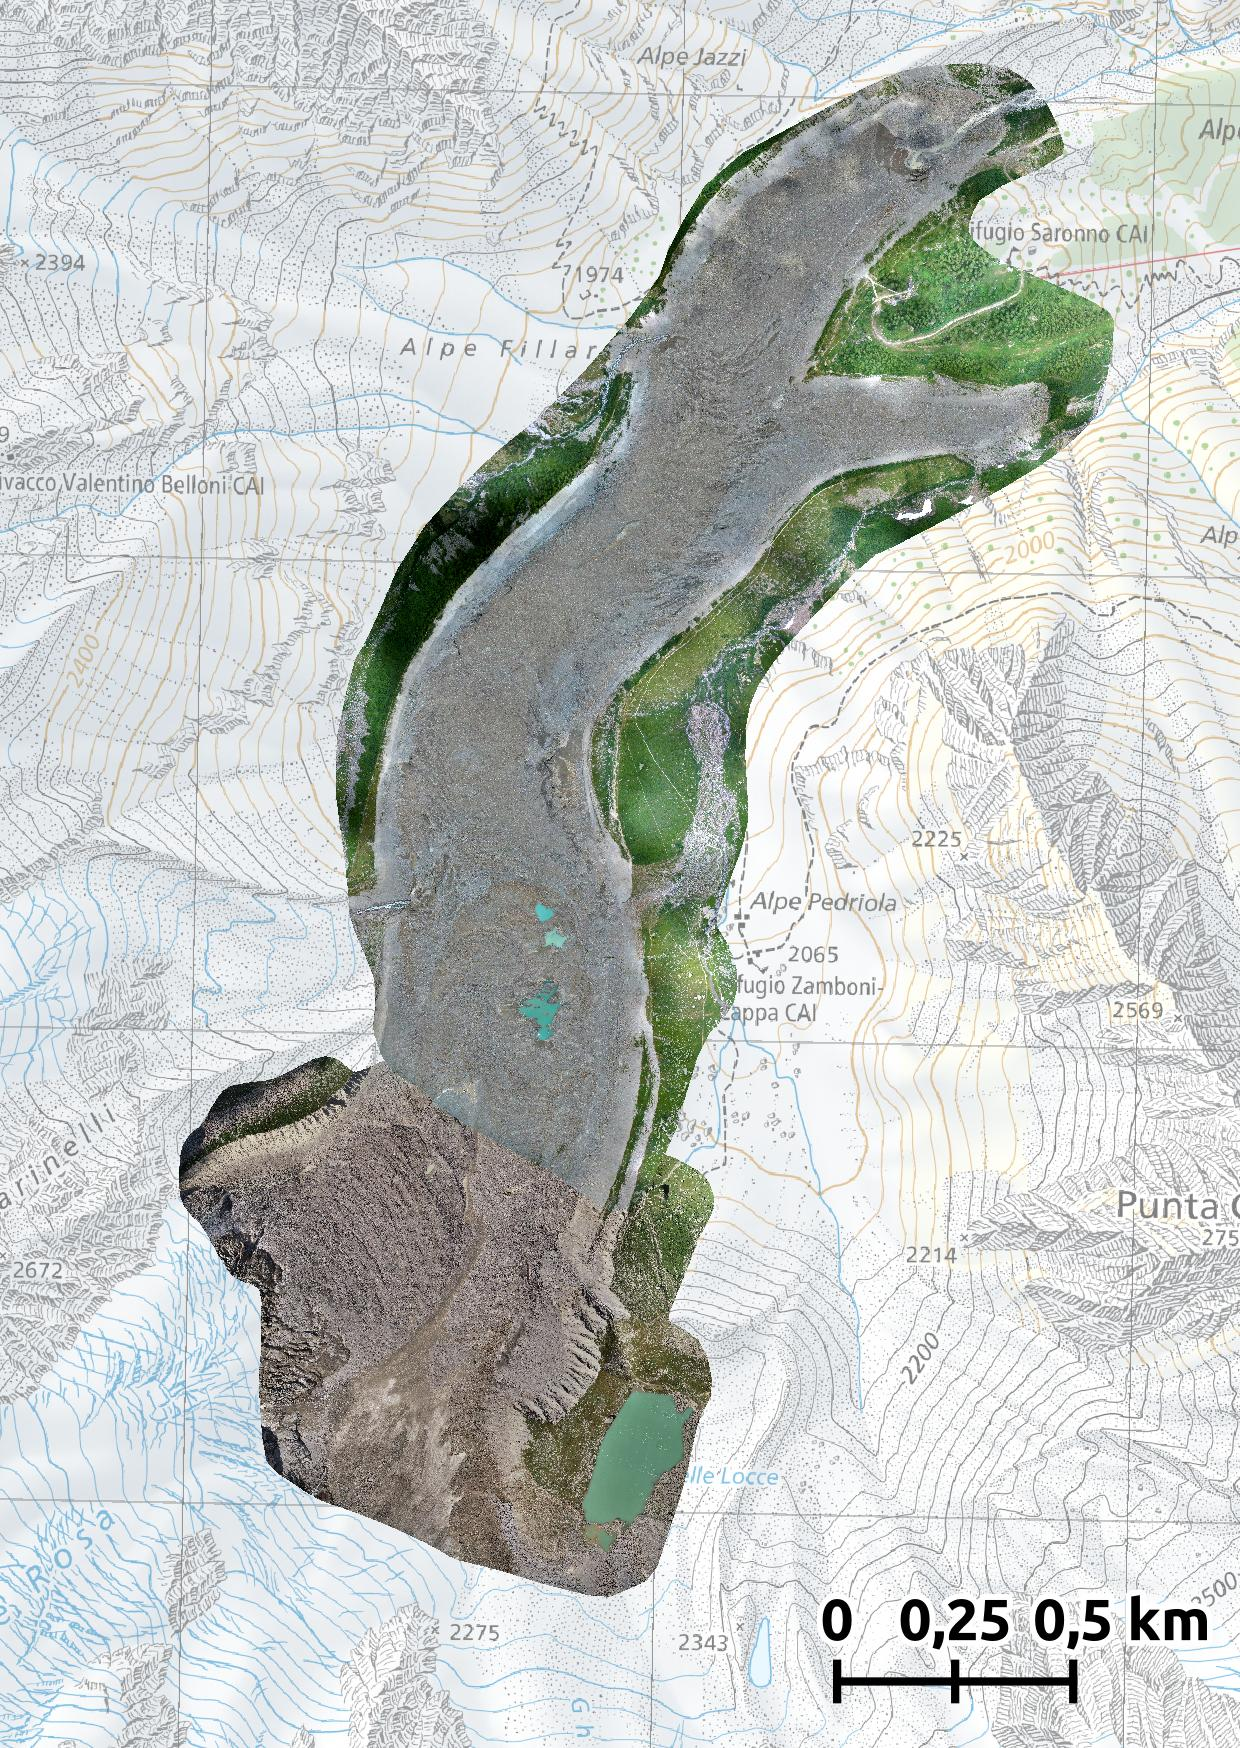
\includegraphics[width=0.30\textwidth]{orto2020.jpg}
    }
    \subcaptionbox{\label{fig:3:ortophoto:2021}}{
        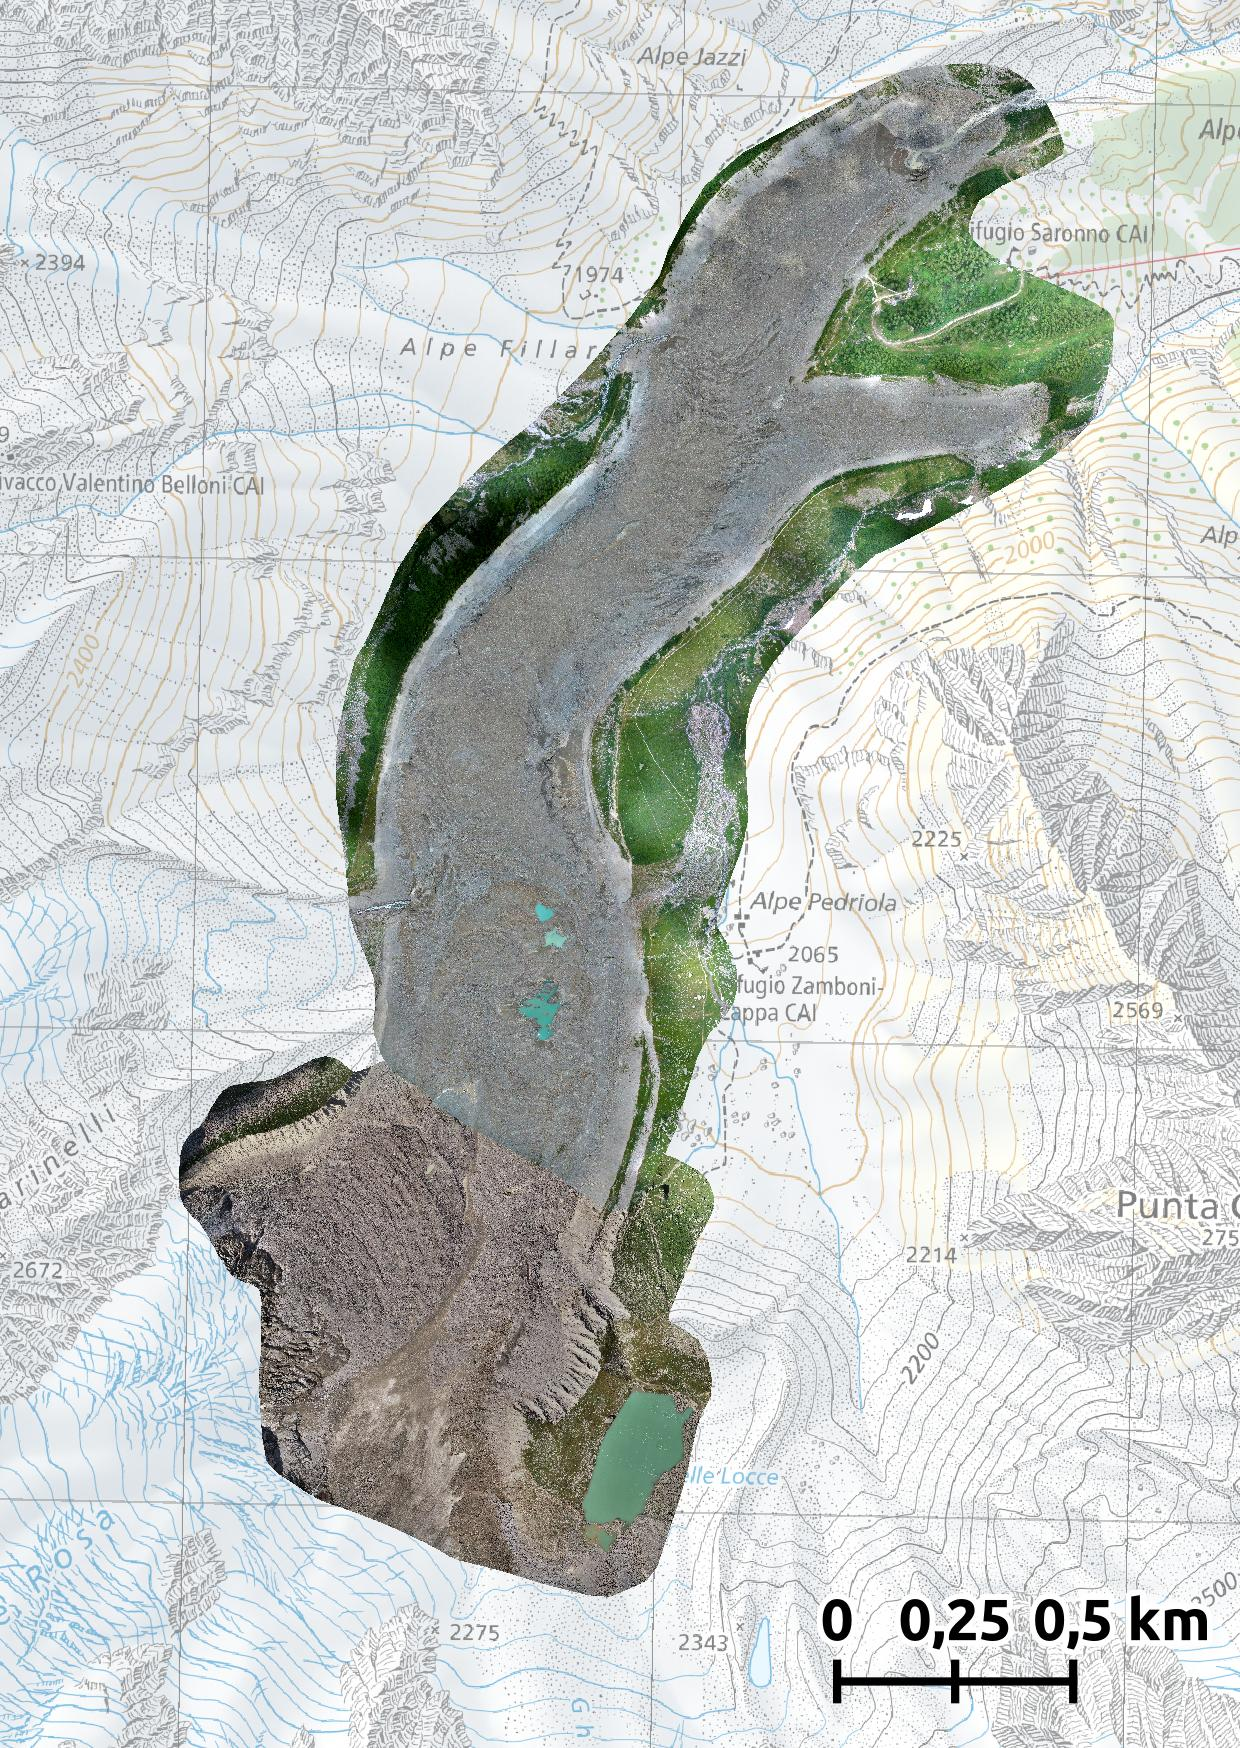
\includegraphics[width=0.30\textwidth]{orto2020.jpg}
    }
    \subcaptionbox{\label{fig:3:ortophoto:2022}}{
        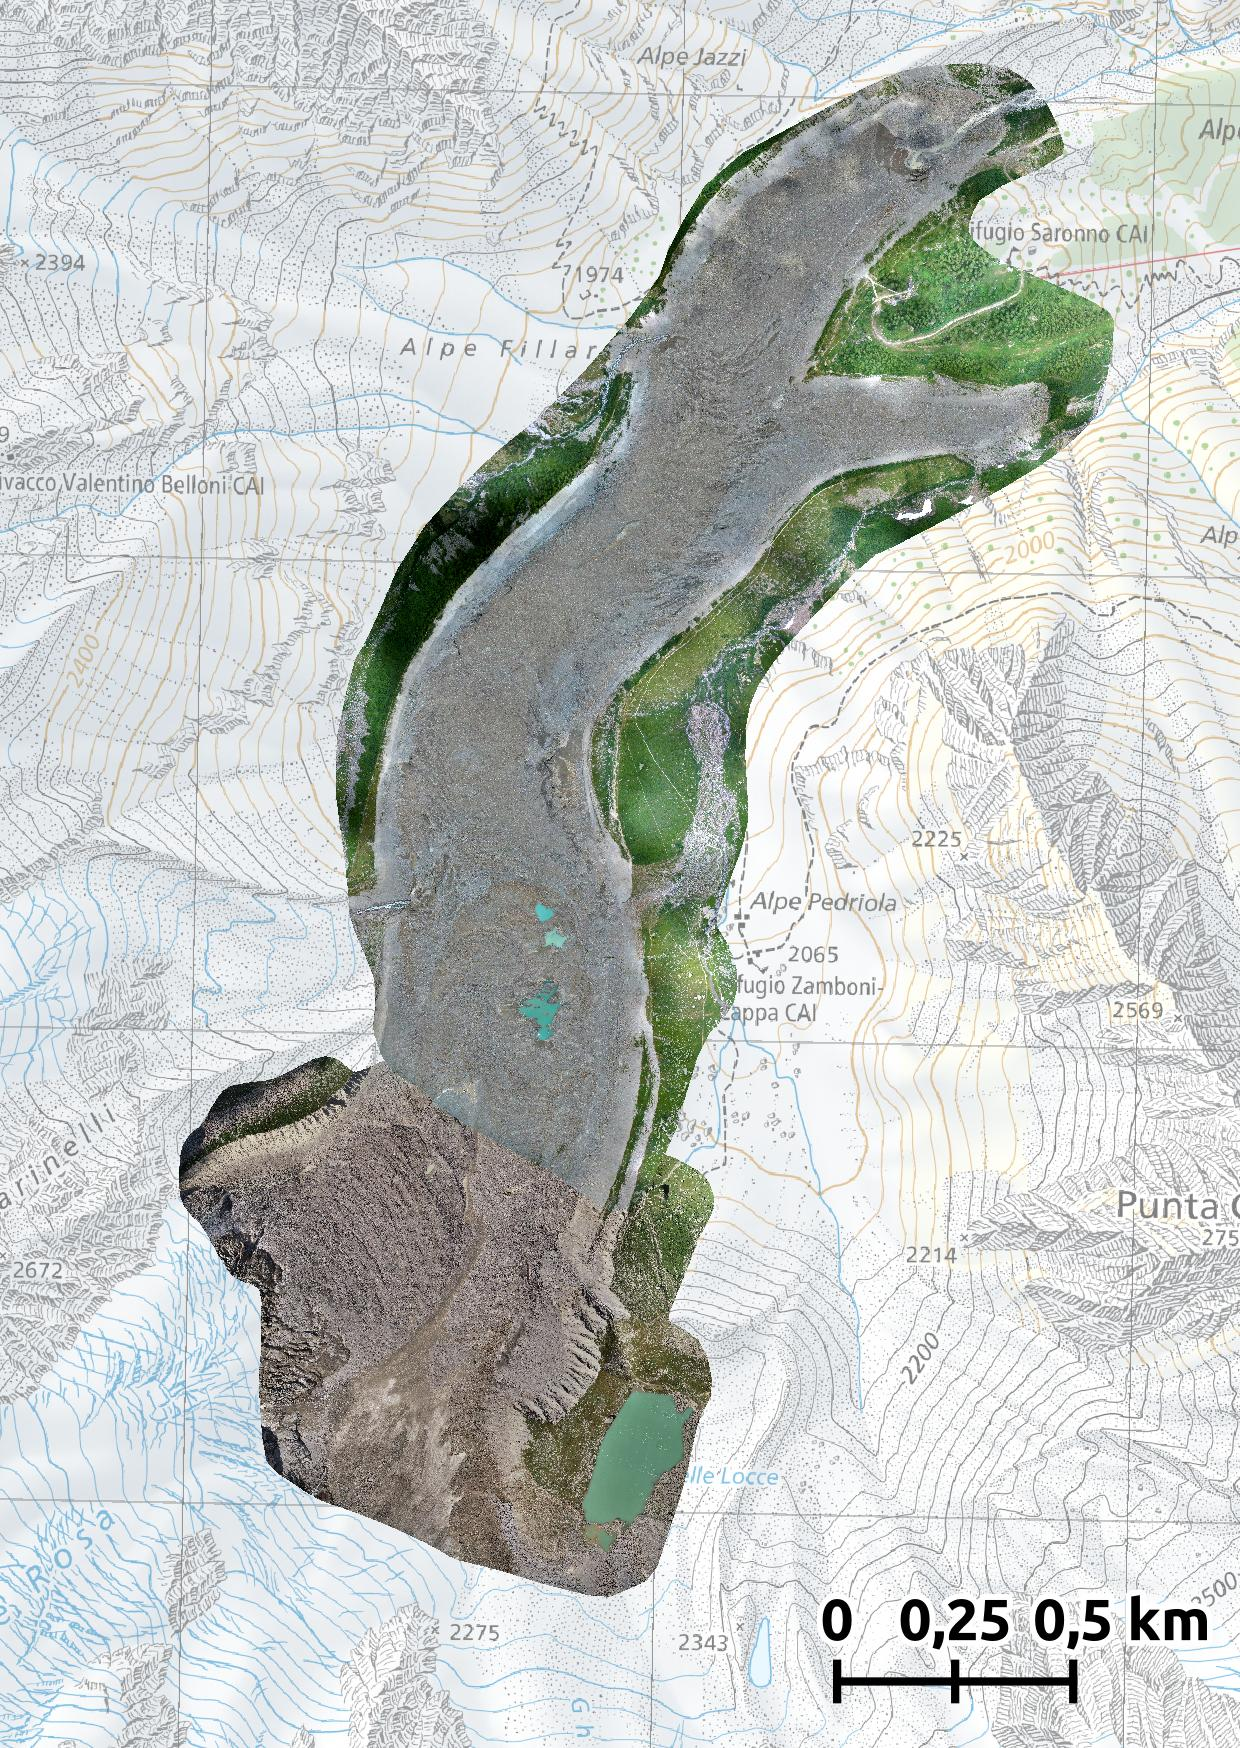
\includegraphics[width=0.30\textwidth]{orto2020.jpg}
    }
    \subcaptionbox{\label{fig:3:ortophoto:2023}}{
        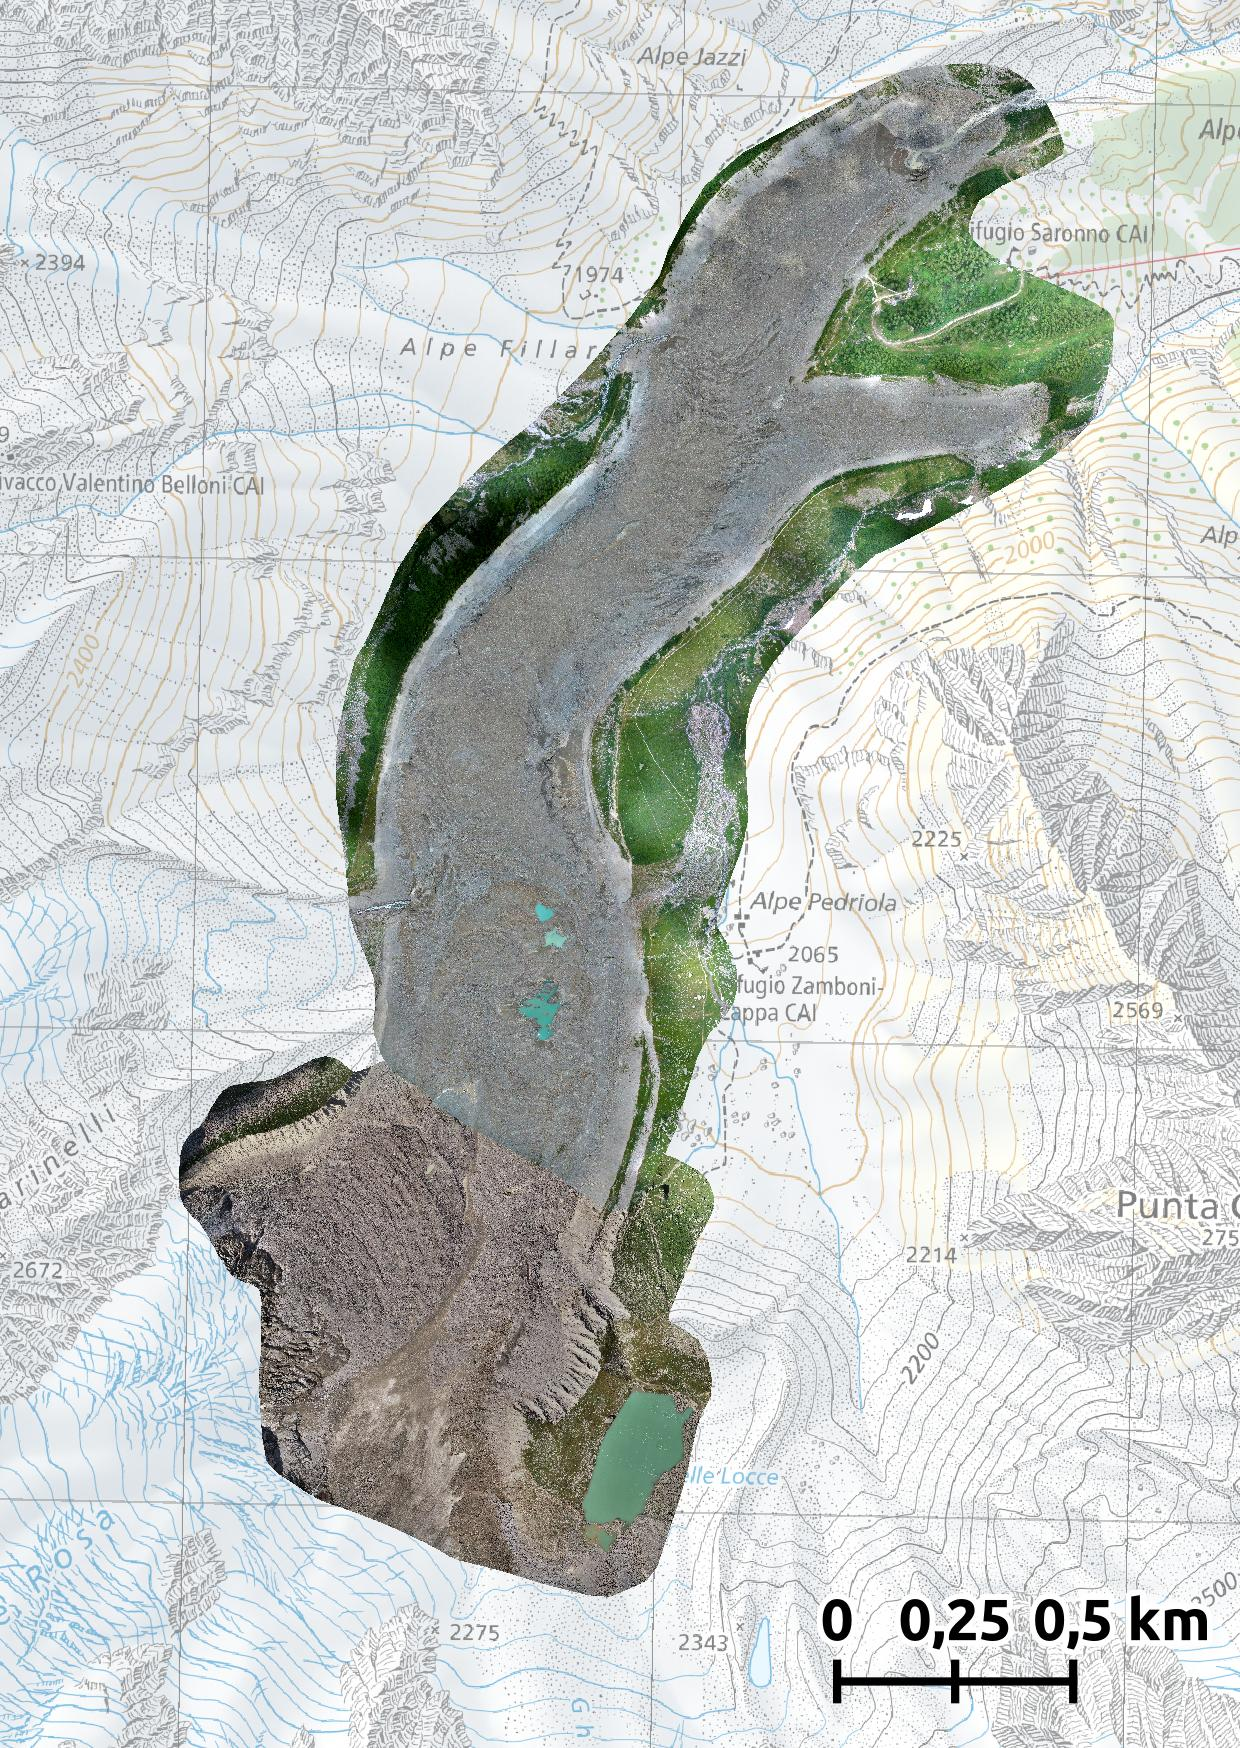
\includegraphics[width=0.30\textwidth]{orto2020.jpg}
    }
    \caption{Orthophotos obtained from the photogrammetric model for each year.
        (\textbf{a}) 2015, (\textbf{b}) 2016, (\textbf{c}) 2017, (\textbf{d}) 2018,
        (\textbf{e})
        2019, (\textbf{f}) 2020, (\textbf{g}) 2021, (\textbf{h}) 2022, (\textbf{i})
        2023. {\color{red} Add recent years}}
    \label{fig:3:ortophoto}
\end{figure}

The re-projection RMSE over the CPs are shown in \figref{fig:3:CP_errors} as assessment
of the geometrical accuracy of the models.
The global re-projection RMSE was mostly ranging between \SIlist{0.1;0.2}{\meter}.
The only exception consisted in the {\color{red} upper sector (comparable to sector S1 in
\figref{fig:3:belvedere}a) of the 2020 model}, for~which the RMSE is almost double
compared to the other values.
{\color{red}
This was caused by practical problems occurred in 2020, explained in detail in
\secref{sec:3:problems}.
}
As a consequence, the~value of 2020 RMSE was split in two different bars in the graph.
From 2015 to 2017, when compact cameras were used, errors comparable to 1.5 times the GSD
were obtained.
Since 2018, a~lightweight action-cam has been employed to minimize the UAV take-off
weight and this has led to an RMSE up to 3~times the GSD, but~still always smaller than
\SI{0.2}{\meter}.

\subsection{Glacier flow velocity\textcolor{red}{TODO}}\label{sec:3:res:velocity}

Annual ice flow velocities were first computed from in-situ GNSS measurements of \textit{moving targets}.
\figref{fig:3:GNSS_velocity} shows the time-series of the velocities of GNSS points. 
Most of the moving targets were found and measured for 3 or more years and some of them have been continuously tracked since 2015 (e.g., the point \textit{M10} in the upper part of the glacier, \textit{M28} in the middle part or \textit{M41} on the south-east tongue). 
However, some of them have been lost over the year, e.g. because they fell into a crevasse, and they were replaced with new ones. 
The location accuracy of the GNSS measurement was estimated as \qty{\sim 3}{\centi\meter} (see Section~\ref{sec:3:gnss}). 
Assuming measurements of the same GCPs at two consecutive years as independent,
the expected standard deviation of the velocity was computed by propagating the variance as \qty{\pm 0.04}{\meter\per\year} (i.e., two order of magnitude less than the computed annual velocities which ranges between \qtylist{2;22}{\meter\per\year}).
Therefore, GNSS measurement are considered as the reference source of information for flow velocity estimation.

From graph in \figref{fig:3:GNSS_velocity}, GNSS points can be visually grouped in three clusters (C1, C2, C3) on the basis of velocity magnitude. 
The first low-velocity cluster C1 includes points with velocities between  \qtylist{2;7}{\meter\per\year}. 
{\color{red}
The location of GNSS points included in C1 well match morphological sectors S1 (upper accumulation sector) and S3 (glacier tongues), marked in \textcolor{red}{FIGXX}.
% \figref{fig:belvedere}a.
By contrast, cluster C3 presents significantly higher speed, ranging between \qtylist{17;22}{\meter\per\year} were sensed in the central sector S2 (e.g., \textit{M10, M11, M22, M28}).
Cluster C2 include GNSS points located in transition areas between S2 and S1 (e.g., targets \textit{M10, M11}, placed between the central sector and the accumulation area) and between S2 and S3 (e.g., \textit{M49}, between the central sector and the lower north-west tongue).
}

{\color{red} Move to discussion: 
Measurements of targets \textit{M22, M23} and \textit{M28} suggests the presence of a rising velocity trend in the central part of the glacier between 2018 and 2020. 
In fact, these points experienced an increase of the velocity magnitude of \qty{\sim 1}{\meter\per\year} from 2018 to 2020.
However, some more measurement years would be necessary to state if this increasing velocity trend holds and is significant. 
On the other hand, all the other targets showed rather steady velocities over the 6 years.
}

\begin{figure}
    \subcaptionbox{\label{fig:3:GNSS_velocity:ts}}{
        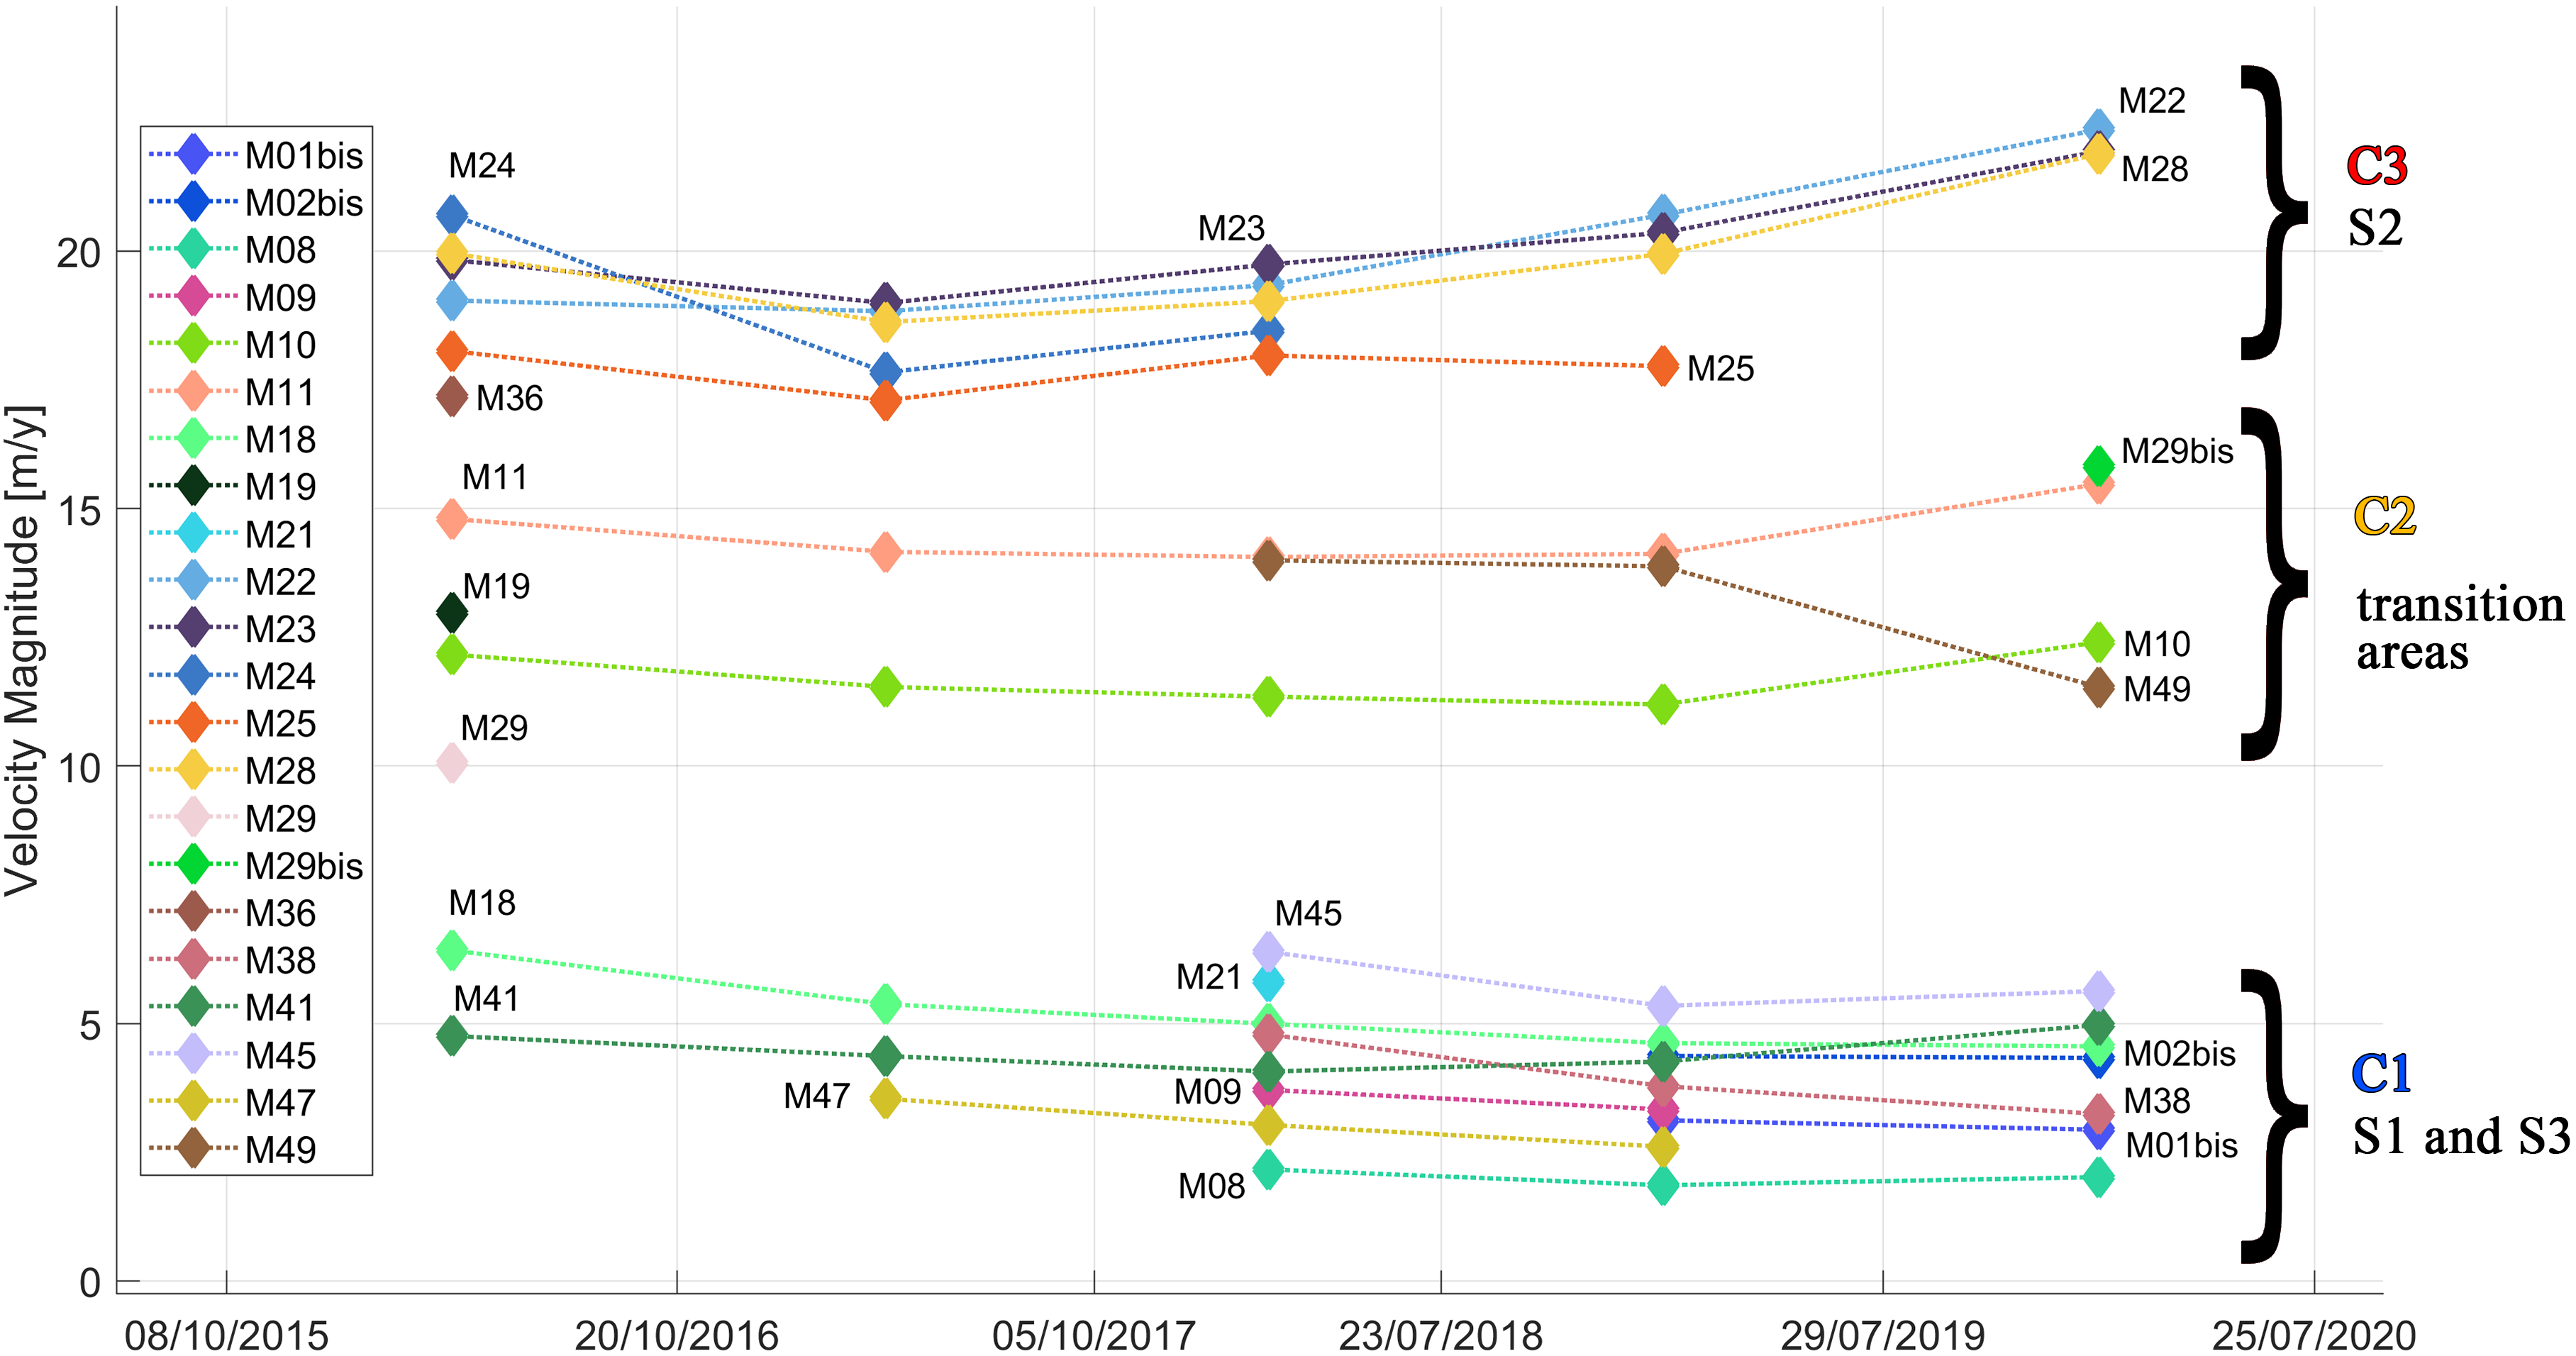
\includegraphics[width=0.68\textwidth]{GCPghiacciaioSerieTemp_02}
    }
    \subcaptionbox{\label{fig:3:GNSS_velocity:map}}{
        \includegraphics[width=0.29\textwidth]{GCPghiaccaio_clusters}
    }
    \caption{\textbf{(a)} Time series of the velocity computed from the GNSS measurements of the targets deployed over the glacier. Dashed lines denote measurement continuity over the years (i.e., if the line is interrupted, the target was lost or not measured during that year). Labels C1-C3 denote the three velocity clusters of GNSS points, whereas labels S1-S3 indicate the three morphological sectors marked in \figref{fig:belvedere}a. A correspondence between clusters and sectors can be identified: C1 corresponds to sectors S1 and S2, cluster C3 to sector S2, whereas cluster C2 corresponds to the two transition areas S2-S1 and S2-S3. \textbf{(b)} Location of the targets over the glacier.}
    \label{fig:3:GNSS_velocity}		
\end{figure}

\subsection{Volume variations \textcolor{red}{Update}}\label{sec:3:res:volumes}

{\color{red} Add 2021-2023!}

\begin{figure}
    \centering
    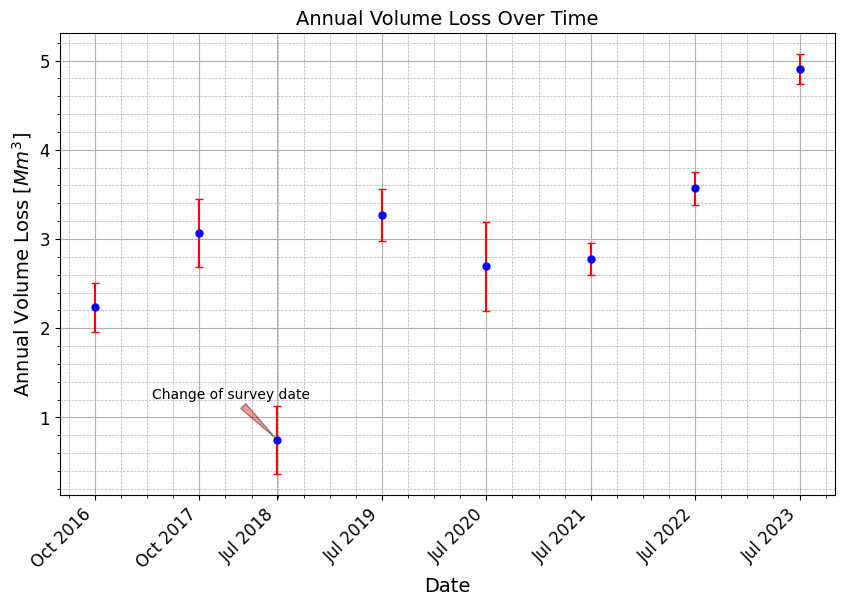
\includegraphics[width=0.8\columnwidth]{volume_loss_2015-2023.png}
    \caption{Yearly volume variation computed as difference between DSM of two
        consecutive years. The~error bars plotted represent the uncertainty of each
        estimated value. Note that the values on the Y axis are expressed in million of
        \si{\cubic\meter}.}
    \label{fig:3:volumes}
\end{figure}

\figref{fig:3:volumes} illustrates the loss of ice volume year by year.
The estimated variance of the glacier volume variation is plotted as an error bar for
each value of volume~variation.

Between 2017 and 2018, field works were moved from Autumn to Summer.
Therefore, the~loss of volume for the year 2017--2018 was computed between October 2017
and July 2018, therefore it represented only the variation occurred in wintertime and
springtime, and~it should not be directly compared with the annual average.
Indeed, 2017--2018 volume variation was \SI{-0.75e6}{\cubic\meter}, against~the average
variation between 2015 and 2020 of \SI{-2.81e6}{\cubic\meter} (difference of
\SI{27}{\percent}).
Ice volume loss for the year 2019--2020 may be slightly underestimated as well: the
photogrammetric model of the upper part of the glacier was affected by a larger geometric
(RMSE in vertical direction of \SI{0.28}{\meter}, see \secref{sec:3:problems})
compared to the others models, due to the lack of GCPs measured in-situ at the time of
the photo acquisition.
Overall, the~negative ice volume variation occurred between 2015 and 2020 is evident and
significant: every year, between~\SIlist{2e6;3.5e6}{\cubic\meter} of ice were~lost.

\begin{figure}
  \centering
  \subcaptionbox{\label{fig:3:profiles:AA}}{
    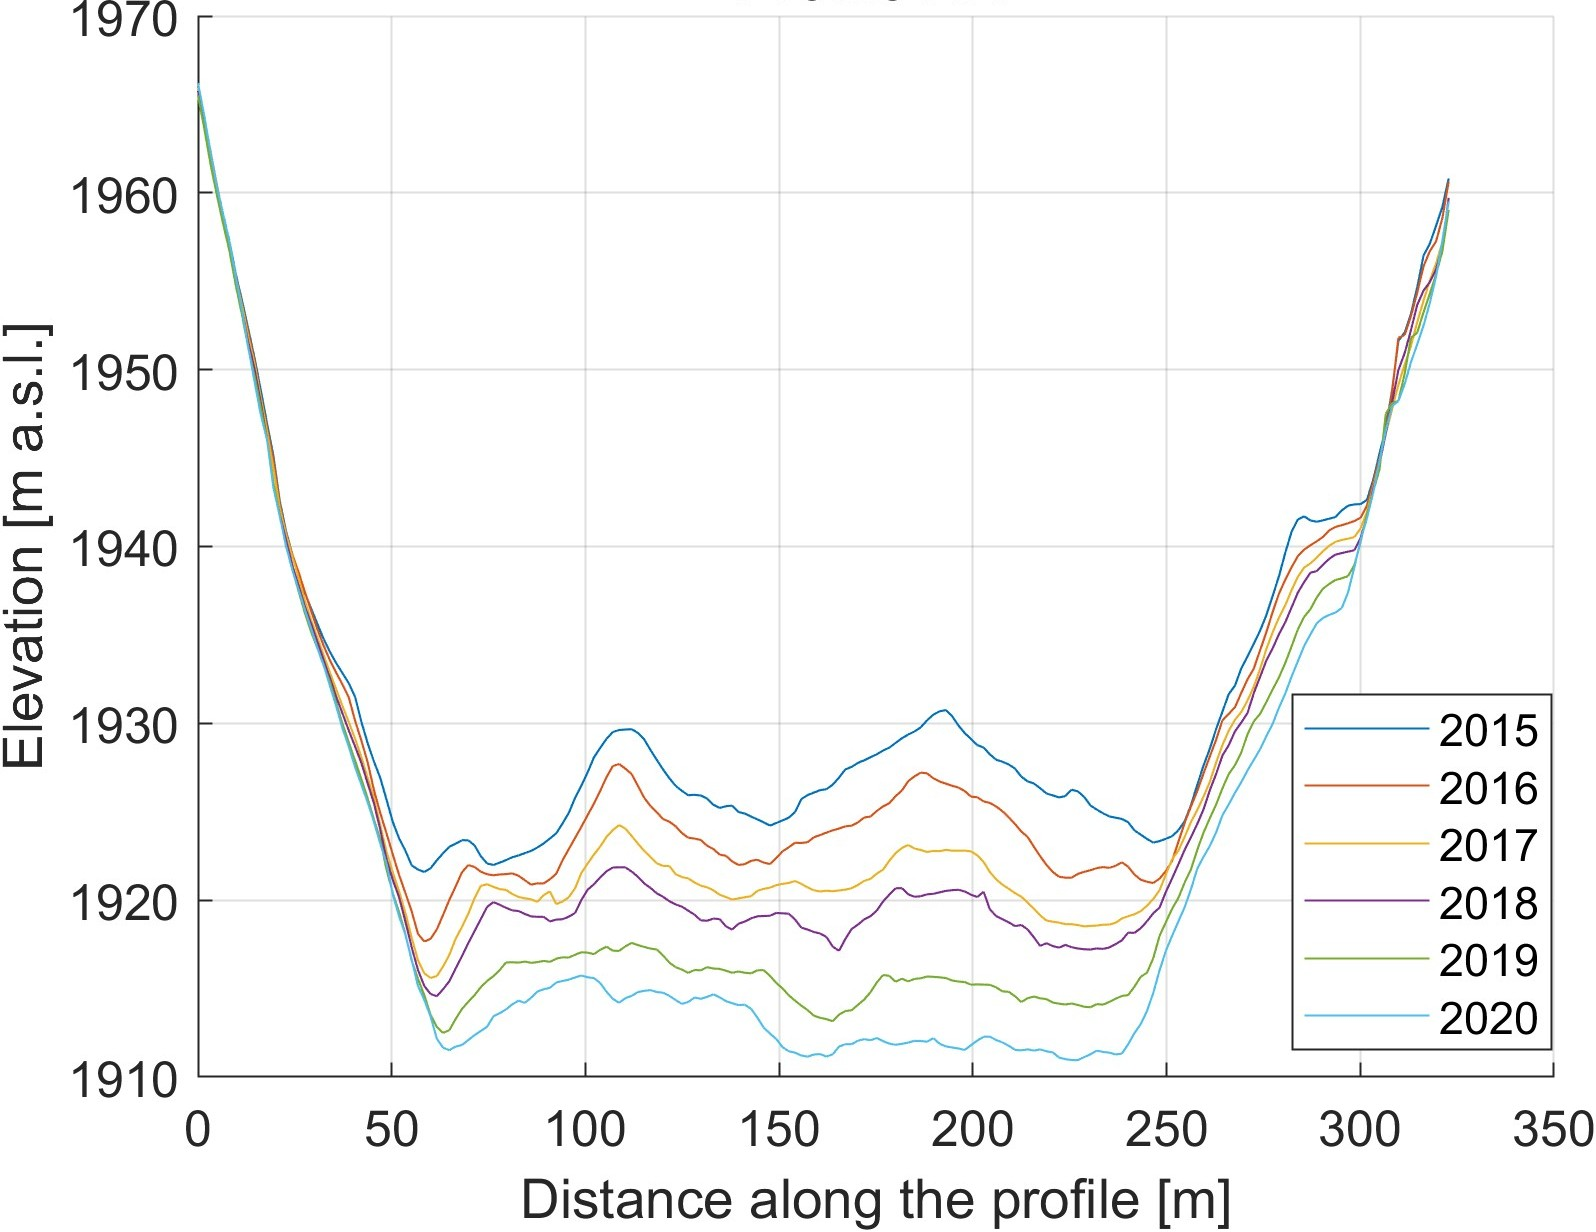
\includegraphics[width=.45\textwidth]{profile_AA.jpg}
  }
  \subcaptionbox{\label{fig:3:profiles:BB}}{
    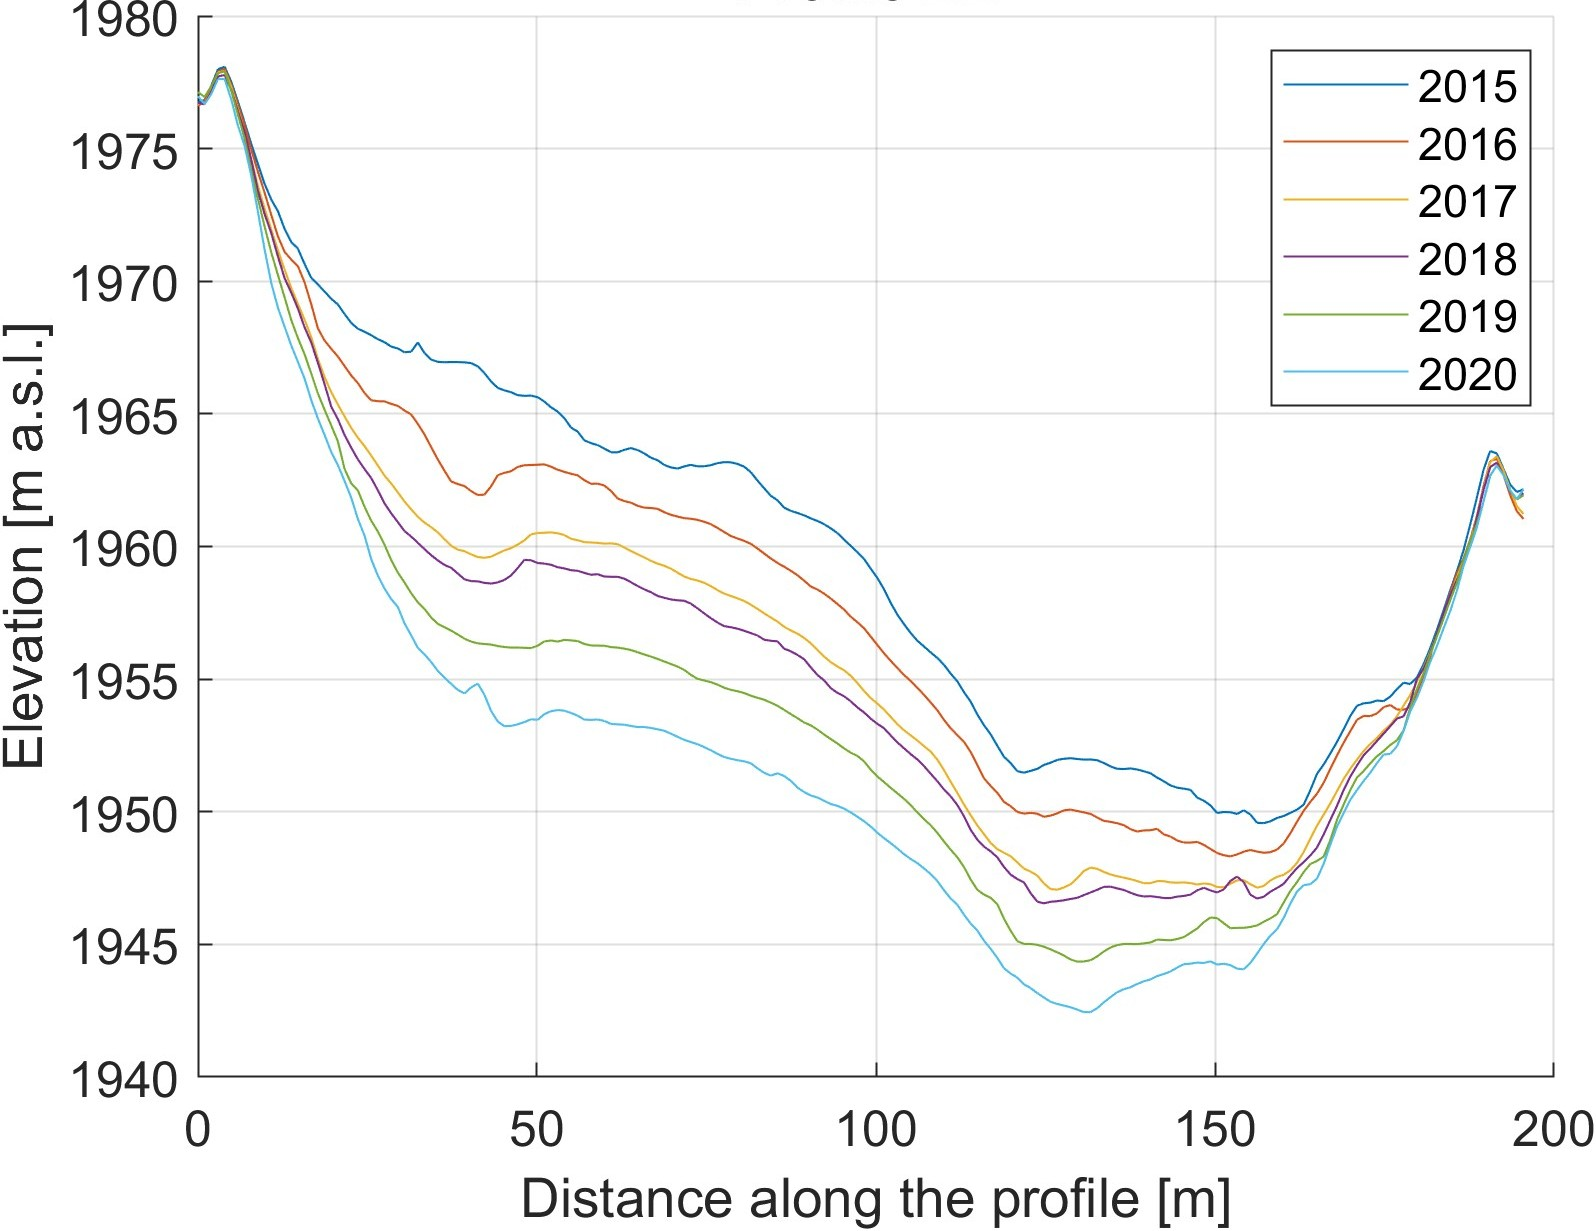
\includegraphics[width=.45\textwidth]{profile_BB.jpg}
  }\\
  \subcaptionbox{\label{fig:3:profiles:CC}}{
    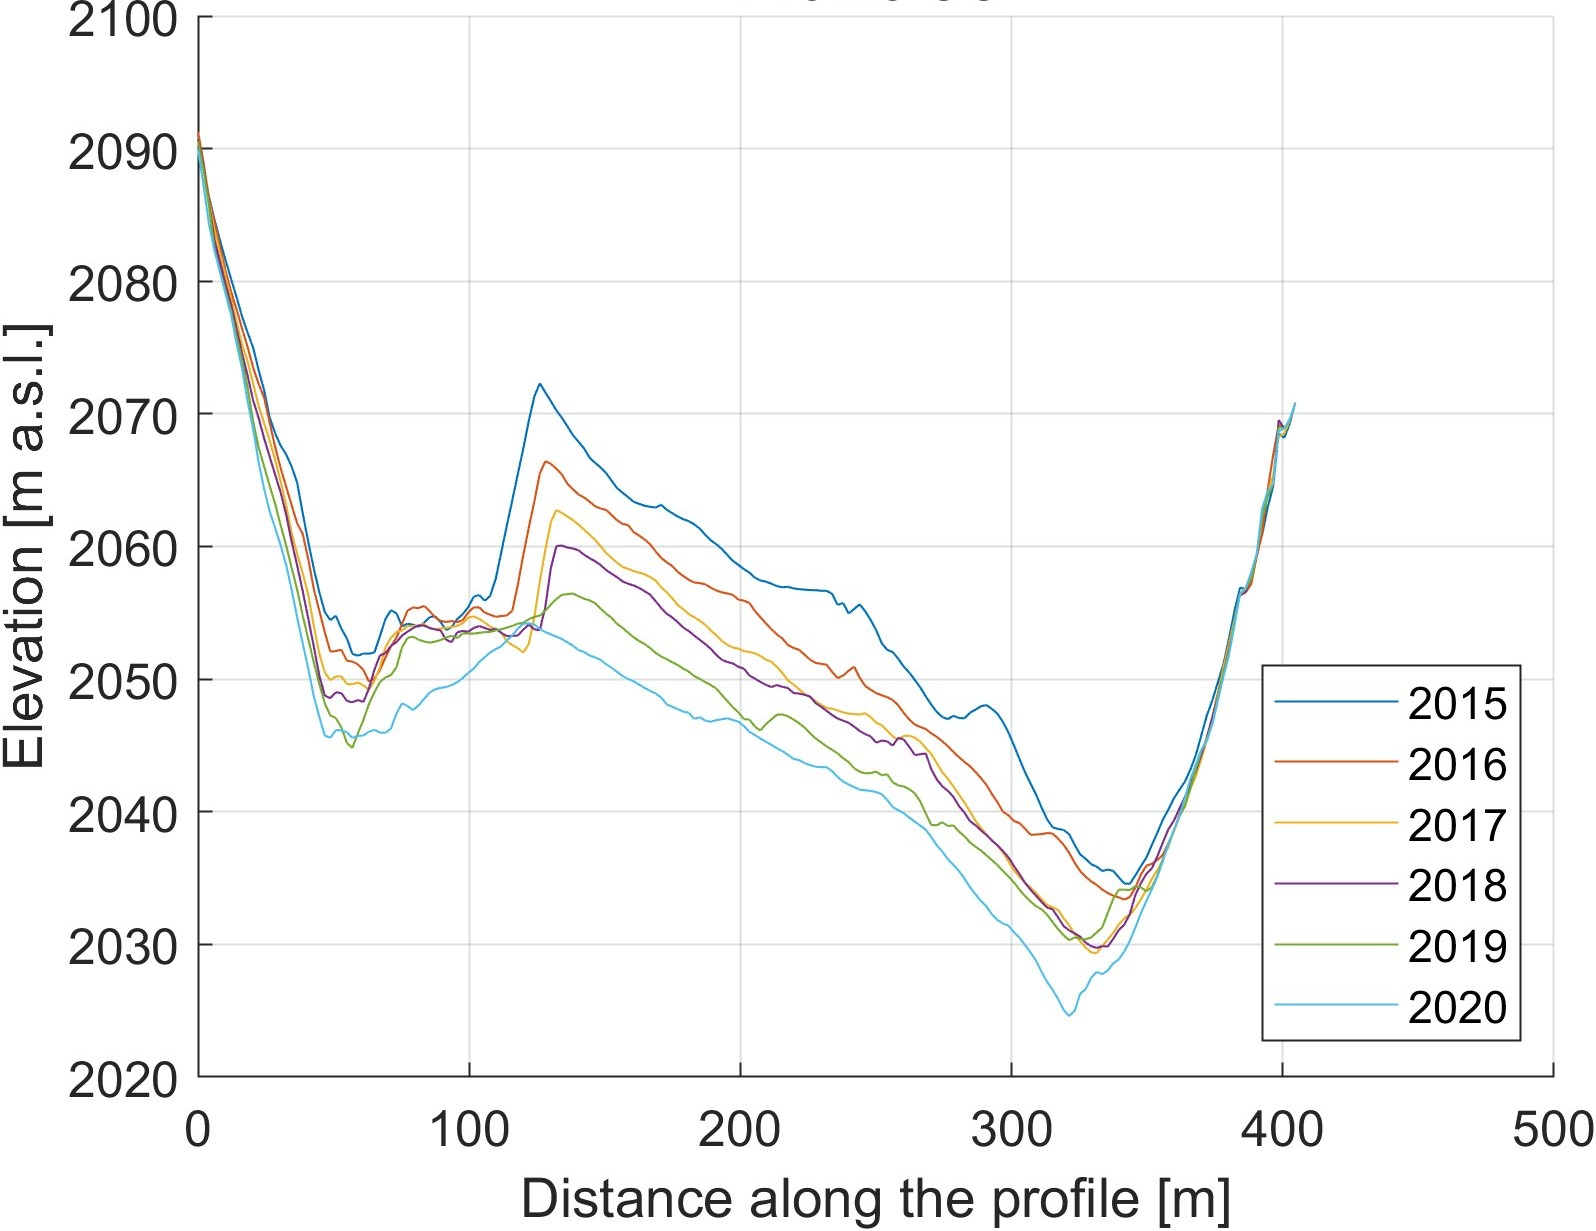
\includegraphics[width=.45\textwidth]{profile_CC.jpg}
  }
  \subcaptionbox{\label{fig:3:profiles:DD}}{
    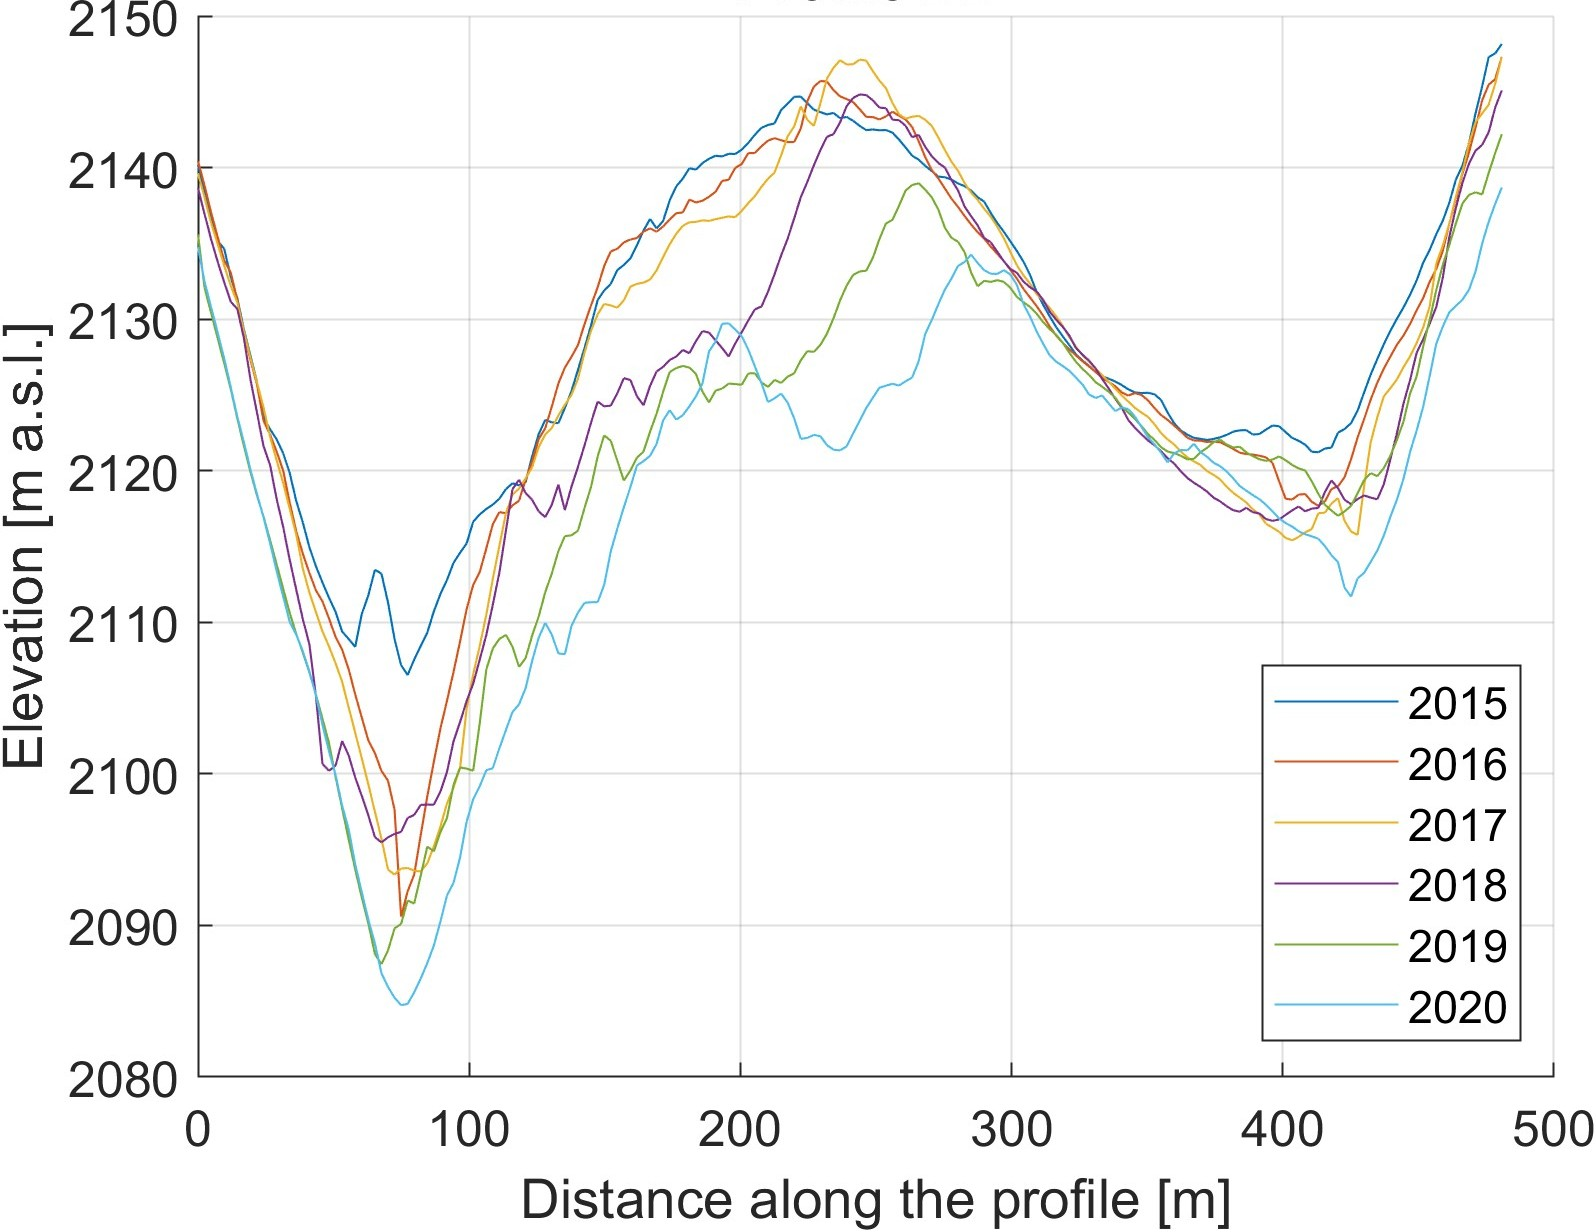
\includegraphics[width=.45\textwidth]{profile_DD.jpg}
  } \\
  \subcaptionbox{\label{fig:3:profiles:map}}{
    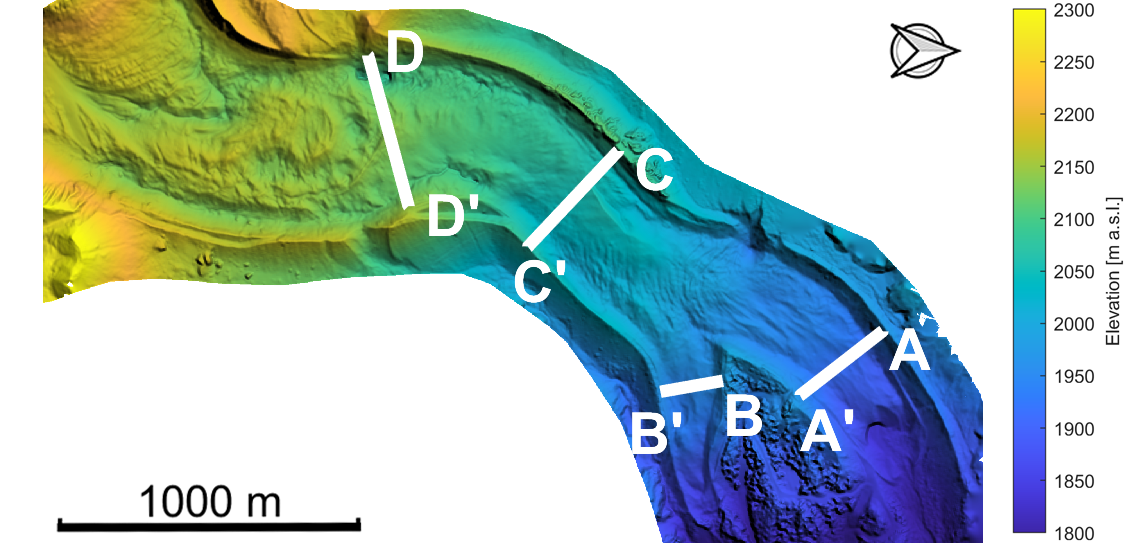
\includegraphics[width=.45\textwidth]{profileMap.png}
  }
    \caption{Elevation profiles obtained from the DSM computed on the years 2015-2020 along 4 different cross-sections. \textbf{(a)} Cross-section AA' at the north-west glacier tongue; \textbf{(b)} Cross-section BB' at the south tongue; \textbf{(c)} Cross-section CC' in the lower portion of the glacier transition sector; \textbf{(d)} Cross-section DD' in the upper portion of the glacier transition sector; \textbf{(e)} Cross-sections location. Cross-sections are seen from South towards North (i.e., from upstream to downstream of the glacier), as marked by the letters in \textbf{(e)}.}
    \label{fig:3:profiles}
\end{figure}

In \figref{fig:3:profiles}, elevation profiles of the glacier obtained every year at four different cross sections are plotted together.
In each profile, it is easily identifiable the glacier surface, which is delimited by the lateral moraines.
The highest height reduction is found at the lower terminus of the glacier (\figref{fig:3:profiles}a-b): \qty{\sim 2}{\meter} have been lost every year. 
It is noticeable that the overall glacier surface profile remained the same, but the ice thickness shrank.
In the central part of the glacier (sections CC' and DD', \figref{fig:3:profiles}c-d), the height reduction was less regular because of the crevasses that strongly ripple the transfer zone of the glacier.	

\subsection{Glacier outline \textcolor{red}{TODO}}\label{sec:3:res:outline}

{\color{red} TODO}

\section{An open source database to store and share the monitoring results \textcolor{red}{TODO}}

{\color{red} TODO}

\section{Discussion}\label{sec:3:discussion}

\subsection{Morphological sectors\textcolor{red}{TODO}}\label{sec:3:discussion:sectors}

\begin{figure}
    \centering
    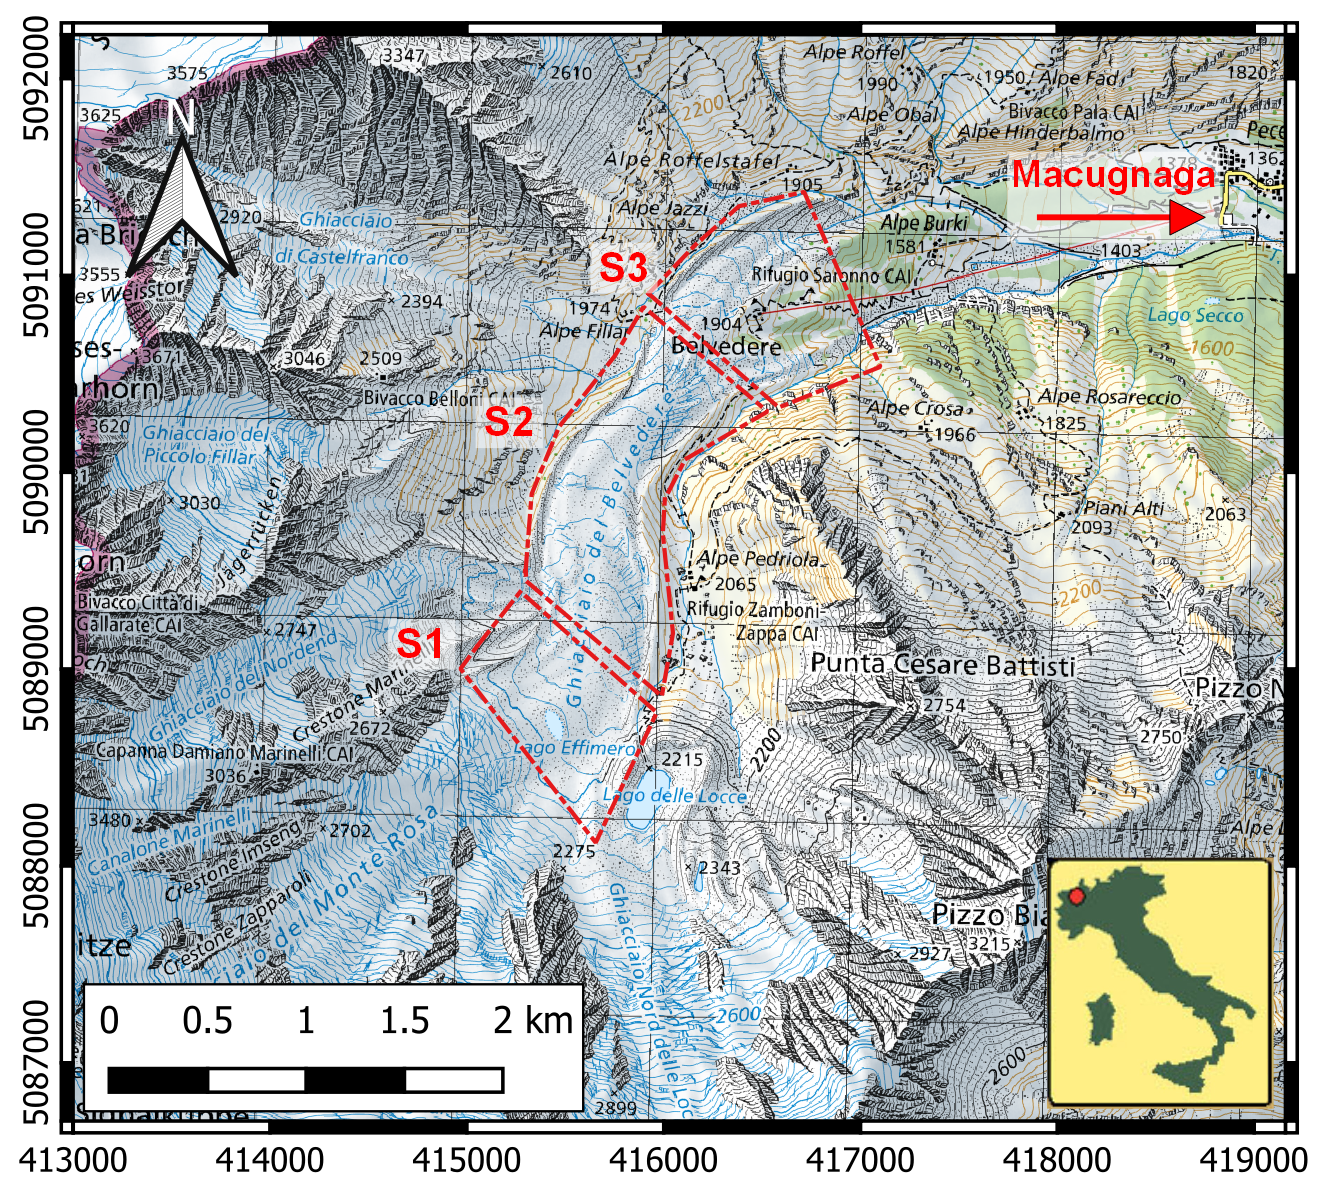
\includegraphics[width=.7\textwidth]{belvedereMapSect}
	\caption{Subdivision of the Belvedere Glacier in three main morphological sectors: sector 1 (S1) is the accumulation zone, sector 2 (S2) is the transfer zone, sector 3 (S3) is the low-relief zone with the two glacier tongues. Coordinates are framed in ETRF2000(2008) UTM 32N. [Basemap source: \textit{Swisstopo (geo.admin.ch)}].}
	\label{fig:3:sectors}	
\end{figure}	

\subsection{Comparison with previous studies\textcolor{red}{UPDATE}}\label{sec:3:discussion:prevstudies}

Several studies focused on understanding and quantifying Belvedere Glacier
dynamics.~\cite{Kaab2005} estimated velocities ranging between
\SIlist{32;43}{\meter\per\year} on the whole Belvedere Glacier from October 1995 to
September 1999, by~employing aerial images.
Besides, velocities between \SIlist{100;200}{\meter\per\year} were estimated
by~\cite{Kaab2005} in Autumn 2001, during~the extraordinary surge event of 2000--2001.
Nowadays, the~Belvedere Glacier is clearly moving slower compared to the late 1990s.
However, to~the best of authors knowledge, there are no recent works estimating glacier
flow~velocities.

Concerning volume variations,~\cite{Diolaiuti2003} digitalized two large-scale
topographic maps to interpolate DSMs and estimate volume variations between 1957 and
1991.
They found a positive volume difference of
\SI[retain-explicit-plus]{+22.7e6}{\cubic\meter} (with an average rate of \SI{\sim
    0.69e6}{\cubic\m\per\year}, roughly assuming a linear volume variation during the
years).

Their result matched with the study of~\cite{Roethlisberger1985}, who estimated an
increase of the glacier height of \SI[retain-explicit-plus]{+1.5}{\m\per\year} between
1983 and 1985.
Recently,~\cite{Degaetani2021} used historical aerial images and UAVs to
photogrammetrically reconstruct glacier volume variations between 1977 and 2019.
For the period 1977--1991, they confirmed the glacier expansion, with~a volume
increase of \SI[retain-explicit-plus]{+10.06e6}{\cubic\meter}
(\SI[retain-explicit-plus]{+0.72e6}{\cubic\m\per\year}).
The expansion continued up to 2001 (at the end of the surge event), with~additional
\SI{10.61e6}{\cubic\m} of ice gained.
Since 2001, a~severe glacier retreat has begun, with~a loss of ice volume of
\SI{-47.78e6}{\cubic\meter} (\SI{-5.97e6}{\cubic\meter\per\year}) between 2001 and 2009.
For the time-span 2009--2019,~\citep{Degaetani2021} derived a negative variation of
\SI{-27.16e6}{\cubic\m} of ice (\SI{-2.72e6}{\cubic\meter\per\year}).
This last ten-years-averaged estimate well matches with the annual volume variations
found in this study between 2015 and 2020 (between
\SIlist{-2e6;-3.5e6}{\cubic\meter\per\year}).



% References
\makechapterbibliography{}

